\section{{\tt Parse::Yapp}: Ejemplo de Uso}
\label{section:ejemplodeuso}
El generador de analizadores sintácticos \tei{Parse::Yapp} es un
analizador LALR inspirado en \tei{yacc}. El módulo
\verb|Parse::Yapp| no viene con la distribución de Perl, por lo que es necesario
bajarlo desde CPAN, en la dirección 

\begin{latexonly}
\begin{verbatim}
\http://search.cpan.org/~fdesar/Parse-Yapp-1.05/lib/Parse/Yapp.p
\end{verbatim}
\end{latexonly}

\begin{rawhtml}
<a href="http://search.cpan.org/~fdesar/Parse-Yapp-1.05/lib/Parse/Yapp.pm">http://search.cpan.org/~fdesar/Parse-Yapp-1.05/lib/Parse/Yapp.pm</a> 
\end{rawhtml}

o bien en nuestros servidores locales,
por ejemplo en el mismo directorio en que se guarda
la versión HTML de estos apuntes encontrará una copia de 
\htmladdnormallink{Parse-Yapp-1.05.tar.gz}{Parse-Yapp-1.05.tar.gz}.
La versión a la que se refiere este capítulo es la 1.05.


Para ilustrar su uso veamos
un ejemplo en el que se genera una sencilla calculadora numérica. 
Los contenidos del programa \tei{yapp} los hemos guardado
en un fichero denominado \verb|Calc.yp|
(el código completo figura en el apéndice 
en la página \pageref{apendice:calcyp})

\begin{verbatim}
 1  #
 2  # Calc.yp
 3  # 
 4  # Parse::Yapp input grammar example.
 5  #
 6  # This file is PUBLIC DOMAIN 
 7  #
 8  #
\end{verbatim}
Se pueden poner comentarios tipo Perl o tipo C (\verb|/* ... */|)
a lo largo del fichero.
\begin{verbatim}
 9  %right  '='
10  %left   '-' '+'
11  %left   '*' '/'
12  %left   NEG
13  %right  '^'
14  
15  %%
16  input:  #empty
17       |   input line  { push(@{$_[1]},$_[2]); $_[1] }
18  ;
\end{verbatim}
las declaraciones \tei{\%left} y \tei{\%right} expresan la asociatividad
y precedencia de los terminales, permitiendo decidir que árbol construir 
en caso de  ambiguedad. 
\emph{ Los terminales declarados en líneas 
posteriores tienen mas prioridad que los declarados en las líneas anteriores}.
Véase la sección \ref{section:prioridades} para mas detalles.

Un programa \verb|yapp| consta de tres partes: la cabeza, el cuerpo
y la cola. Cada una de las partes va separada de las otras por el
símbolo \verb|%%| en una línea aparte. Así, el \verb|%%| de la línea 15
separa la cabeza del cuerpo. En la cabecera se colocan el
código de inicialización, las declaraciones de terminales, las reglas
de precedencia, etc.  El cuerpo contiene las reglas de la gramática y
las acciones asociadas. Por último, la cola de un program \verb|yapp|
contiene las rutinas de soporte al código que aparece en las acciones 
asi como, posiblemente, rutinas para el análisis léxico 
y el tratamiento de errores.

En \verb|Parse::Yapp| las acciones son convertidas en subrutinas
anónimas. Mas bien en métodos anónimos. 
Así pues el primer argumento de la subrutina se identifica con 
una referencia al analizador (\verb|$_[0]|).  Los restantes parámetros
se corresponden con los \cei{atributos de los símbolos}
en la parte derecha de la regla de producción (\verb|$_[1]| \ldots ).
Por ejemplo, el código en la línea 21 imprime el atributo asociado
con la variable sintáctica \verb|expr|, que en este caso es su valor numérico.

La línea 17 indica que el atributo asociado con la variable
sintáctica \verb|input| es una referencia
a una pila y que el atributo asociado con la variable sintáctica
\verb|line| debe empujarse
en la pila. De hecho, el atributo asociado con \verb|line| es el valor
de la expresión. Asi pues el atributo retornado por \verb|input| es
una referencia a una lista conteniendo los valores de las expresiones
evaluadas.

Para saber mas sobre las estructuras internas de 
\verb|yapp| para la representación  de las acciones asociadas con las reglas
véase la sección \ref{section:tablas}.


\begin{verbatim}
19  
20  line:  '\n'       { 0 }
21      |  exp '\n'   { print "$_[1]\n"; $_[1] }
22      |  error '\n' { $_[0]->YYErrok; 0 }
23  ;
\end{verbatim}

El terminal
\verb|error| en la línea 22 esta asociado con la aparición de un error.
El tratamiento es el mismo que en \verb|yacc|. Cuando se produce un error
en el análisis, \verb|yapp| emite un mensaje de error y
produce ``mágicamente'' un terminal especial denominado
\verb|error|. A partir de ahí permanecerá silencioso,
consumiendo terminales hasta encontrar uno de los terminales que le
hemos indicado en las reglas de recuperación de errores,
en este caso, cuando encuentre un retorno de carro.
Como se ha dicho, en \verb|Parse::Yapp| el primer argumento de la acción denota al 
analizador sintáctico. Así pues el código \verb|$_[0]->YYErrok|
es una llamada al método \verb|YYErrok| del analizador. Este método
funciona como la macro \verb|yyerrok| de \verb|yacc|, indicando 
que la presencia del retorno del carro (\verb|\n|) la podemos considerar
un signo seguro de que nos hemos recuperado del error. A partir
de este momento, \verb|yapp| volverá a emitir mensajes de error.
Para saber más sobre la recuperación de 
errores en \verb|yapp| léase la sección
\ref{section:errores}.

\begin{verbatim}
24  
25  exp:        NUM
\end{verbatim}
La acción por defecto es retornar \verb|$_[1]|. 
Por tanto, en este caso el valor retornado es el asociado a \verb|NUM|.
\begin{verbatim}
26          |   VAR           { $_[0]->YYData->{VARS}{$_[1]} }
\end{verbatim}
El método \verb|YYData| provee acceso a un hash que contiene los datos 
que están siendo analizados. En este caso creamos una entrada
\verb|VARS| que es una referencia a un hash en el que guardamos las
variables. Este hash es la tabla de símbolos de la calculadora.
\begin{verbatim}
27          |   VAR '=' exp   { $_[0]->YYData->{VARS}{$_[1]}=$_[3] }
28          |   exp '+' exp   { $_[1] + $_[3] }
29          |   exp '-' exp   { $_[1] - $_[3] }
30          |   exp '*' exp   { $_[1] * $_[3] }
\end{verbatim}
Hay numerosas ambiguedades en esta gramática. Por ejemplo,

\begin{itemize}
\item
¿Como debo interpretar la expresión \verb|4 - 5 - 2|?
¿Como \verb|(4 - 5) - 2|? ¿o bien \verb|4 - (5 - 2)|?
La respuesta la da la asignación de asociatividad a los operadores
que hicimos en las líneas 9-13.
Al declarar como asociativo a izquierdas al terminal \verb|-| 
(línea 10) hemos 
resuelto este tipo de ambiguedad. Lo que estamos haciendo es
indicarle al analizador que a la hora de elegir entre 
los árboles abstractos 
$-(-(4,5),2)$ y $-(4, -(5,2))$ elija siempre
el árbol que se hunde a izquierdas.
\item
¿Como debo interpretar la expresión \verb|4 - 5 * 2|?
¿Como \verb|(4 - 5) * 2|? ¿o bien \verb|4 - (5 * 2)|?
Al declarar que \verb|*| tiene mayor prioridad que \verb|-| estamos
resolviendo esta otra fuente de ambiguedad. Esto es así pues
\verb|*| fué declarado en la línea 11 y \verb|-| en la 10.
\end{itemize}

\begin{verbatim}
31          |   exp '/' exp   {
32                              $_[3]
33                              and return($_[1] / $_[3]);
34                              $_[0]->YYData->{ERRMSG}
35                                =   "Illegal division by zero.\n";
36                              $_[0]->YYError;
37                              undef
38                            }
\end{verbatim}

En la regla de la división comprobamos que el divisor es 
distinto de cero. Si es cero inicializamos el atributo 
\verb|ERRMSG| en la zona de datos con el mensaje de
error apropiado. Este mensaje es aprovechado por la subrutina
de tratamiento de errores (véase la subrutina \verb|_Error|
en la zona de la cola). La subrutina \verb|_Error| es llamada
automáticamente por \verb|yapp| cada vez que ocurre un error
sintáctico. Esto es asi por que en la llamada 
al analizador se especifican quienes son las diferentes
rutinas de apoyo:

\begin{verbatim}
my $result = $self->YYParse( yylex => \&_Lexer, 
                             yyerror => \&_Error,
                             yydebug => 0x0 );
\end{verbatim}

Por defecto, \emph{una regla de producción
tiene la prioridad del último terminal que aparece
en su parte derecha}.
Una regla de producción puede ir seguida de una directiva
\verb|%prec| la cual le da una prioridad explícita.  
Esto puede ser de gran ayuda en ciertos casos de 
ambiguedad.

\begin{verbatim}
39          |   '-' exp %prec NEG   { -$_[2] }
\end{verbatim}
¿Cual es la ambiguedad que surge con esta regla? 
Una de las ambiguedad de esta regla 
esta relacionada con el doble significado
del menos como operador unario y binario: hay frases
como \verb|-y-z| que tiene dos posibles interpretaciones:
Podemos verla como \verb|(-y)-z| o bien como \verb|-(y-z)|.
Hay dos árboles posibles. El analizador, cuando este analizando
la entrada \verb|-y-z| y vea el
segundo \verb|-| deberá escoger uno de los dos árboles. 
¿Cuál?. El conflicto puede verse como una ``lucha'' entre
la regla \verb|exp: '-' exp| la cual interpreta la frase como
\verb|(-y)-z| y la segunda aparición del terminal \verb|-| 
el cuál ``quiere entrar'' para que gane la regla \verb|exp: exp '-' exp|
y dar lugar a la interpretación \verb|-(y-z)|.
En este caso, las dos reglas 
$E \rightarrow - E$ y $E \rightarrow E - E$ tienen, en principio
la prioridad del terminal \verb|-|, el cual fué declarado en la
línea 10.
La prioridad expresada explícitamente
para la regla por la declaración \verb|%prec NEG| de la línea
39 hace que la regla tenga la prioridad
del terminal \verb|NEG| (línea 12) y por tanto mas prioridad
que el terminal \verb|-|. Esto hará que \verb|yapp| finalmente opte
por la regla \verb|exp: '-' exp|.

La declaración de \verb|^| como asociativo a derechas y con un nivel
de prioridad alto resuelve las ambiguedades relacionadas 
con este operador:

\begin{verbatim}
40          |   exp '^' exp         { $_[1] ** $_[3] }
41          |   '(' exp ')'         { $_[2] }
42  ;
\end{verbatim}

Después de la parte de la gramática, y separada de la anterior
por el símbolo \verb|%%|, sigue la parte en la que se 
suelen poner las rutinas de apoyo. Hay al menos dos rutinas de apoyo que 
el analizador sintáctico requiere le sean pasados como argumentos: 
la de manejo de errores y la de análisis léxico. El método \verb|Run|
ilustra como se hace la llamada al método de análisis sintáctico 
generado, utilizando la técnica de llamada con argumentos con nombre 
y pasándole las referencias a las dos subrutinas (en Perl,
es un convenio que si el nombre de una subrutina comienza
por un guión bajo es que el autor la considera privada):
\begin{verbatim}
...

sub Run {
    my($self)=shift;
    my $result = $self->YYParse( yylex => \&_Lexer, 
                                 yyerror => \&_Error,
                                 yydebug => 0x0 );
    my @result = @$result;
    print "@result\n";
}
\end{verbatim}

La subrutina de manejo de errores \verb|_Error| imprime 
el mensaje de error proveído por el usuario, el cual, si existe, fué guardado en
\verb|$_[0]->YYData->{ERRMSG}|.
\begin{verbatim}
43  # rutinas de apoyo 
44  %%
45  
46  sub _Error {
47    exists $_[0]->YYData->{ERRMSG}
48      and do {
49          print $_[0]->YYData->{ERRMSG};
50          delete $_[0]->YYData->{ERRMSG};
51          return;
52      };
53    print "Syntax error.\n";
54  }
55  
\end{verbatim}
A continuación sigue el método que implanta
el  análisis léxico \verb|_Lexer|.
En primer lugar se comprueba la existencia de
datos en \verb|parser->YYData->{INPUT}|. Si no es el caso, los datos
se tomarán de la entrada estándar:
\begin{verbatim}
56  sub _Lexer {
57    my($parser)=shift;
58  
59    defined($parser->YYData->{INPUT})
60    or  $parser->YYData->{INPUT} = <STDIN>
61    or  return('',undef);
62  
\end{verbatim}
Cuando el analizador léxico alcanza el final de la entrada
debe devolver la pareja \verb|('',undef)|.

Eliminamos los blancos iniciales (lo que en inglés se conoce por
\cei{trimming}):
\begin{verbatim}
63    $parser->YYData->{INPUT}=~s/^[ \t]//;
64  
\end{verbatim}
A continuación vamos detectando los números, identificadores
y los símbolos individuales. El bucle \verb|for ($parser->YYData->{INPUT})|
se ejecuta mientras la cadena
en \verb|$parser->YYData->{INPUT}| no sea vacía, lo que ocurrirá cuando todos 
los terminales hayan sido consumidos.

\begin{verbatim}
65    for ($parser->YYData->{INPUT}) {
66      s/^([0-9]+(?:\.[0-9]+)?)//
67        and return('NUM',$1);
68      s/^([A-Za-z][A-Za-z0-9_]*)//
69        and return('VAR',$1);
70      s/^(.)//s
71        and return($1,$1);
72    }
73  }
\end{verbatim}

\begin{exercise}
\begin{enumerate}
\item ¿Quién es la variable índice en la línea 65? 
\item ¿Sobre quién ocurre el binding en las líneas 66, 68 y 70? 
\item ¿Cual es la razón por la que \verb|$parser->YYData->{INPUT}| se 
ve modificado si no aparece como variable para el binding en las líneas 66, 68 y 70?
\end{enumerate}
\end{exercise}

Construimos el módulo \verb|Calc.pm| a partir del fichero \verb|Calc.yp|
especificando la gramática, usando un fichero \verb|Makefile|:
\begin{verbatim}
> cat Makefile
Calc.pm: Calc.yp
        yapp -m Calc Calc.yp
> make
yapp -m Calc Calc.yp
\end{verbatim}
Esta compilación genera el fichero \verb|Calc.pm| conteniendo el
analizador:
\begin{verbatim}
> ls -ltr
total 96
-rw-r-----    1 pl       users        1959 Oct 20  1999 Calc.yp
-rw-r-----    1 pl       users          39 Nov 16 12:26 Makefile
-rwxrwx--x    1 pl       users          78 Nov 16 12:30 usecalc.pl
-rw-rw----    1 pl       users        5254 Nov 16 12:35 Calc.pm
\end{verbatim}

El script \verb|yapp| es un \emph{frontend} al módulo \verb|Parse::Yapp|.
Admite diversas formas de uso:

\begin{itemize}
\item
{\tt yapp [options] \textit{grammar}[.yp]}

El sufijo {\tt .yp} es opcional.
\item
{\tt yapp \textit{-V}}

Nos muestra la versión:
\begin{verbatim}
$ yapp -V
This is Parse::Yapp version 1.05.
\end{verbatim}

\item
{\tt yapp \textit{-h}}

Nos muestra la ayuda:

\begin{verbatim}
$ yapp -h

Usage:  yapp [options] grammar[.yp]
  or    yapp -V
  or    yapp -h

    -m module   Give your parser module the name <module>
                default is <grammar>
    -v          Create a file <grammar>.output describing your parser
    -s          Create a standalone module in which the driver is included
    -n          Disable source file line numbering embedded in your parser
    -o outfile  Create the file <outfile> for your parser module
                Default is <grammar>.pm or, if -m A::Module::Name is
                specified, Name.pm
    -t filename Uses the file <filename> as a template for creating the parser
                module file.  Default is to use internal template defined
                in Parse::Yapp::Output
    -b shebang  Adds '#!<shebang>' as the very first line of the output file

    grammar     The grammar file. If no suffix is given, and the file
                does not exists, .yp is added

    -V          Display current version of Parse::Yapp and gracefully exits
    -h          Display this help screen

\end{verbatim}

\end{itemize}

La opción \textit{-m module} \mbox{}
da el nombre  al paquete o espacio de nombres o clase encapsulando el
analizador. Por defecto toma el nombre de la gramática.  En el ejemplo
podría haberse omitido.

La opción \textit{-o outfile} \mbox{}
da el nombre del fichero de salida. Por defecto toma el nombre de la gramática,
seguido del sufijo \verb|.pm|. sin embargo, si hemos especificado la opción
\textit{-m A::Module::Name} el valor por defecto será  \emph{Name.pm}.


Veamos los contenidos del ejecutable \verb|usecalc.pl| el cuál
utiliza el módulo generado por \verb|yapp|:
\begin{verbatim}
> cat usecalc.pl
#!/usr/local/bin/perl5.8.0 -w

use Calc;

$parser = new Calc();
$parser->Run;
\end{verbatim}
Al ejecutar obtenemos:
\begin{verbatim}
$ ./usecalc3.pl
2+3
5
4*8
32
^D
5 32
\end{verbatim}
Pulsamos al final \verb|Ctrl-D| para generar el final de fichero.
El analizador devuelve la lista de valores computados la cual es 
finalmente impresa.

¿En que orden ejecuta \verb|YYParse| las acciones? 
La respuesta es que el analizador generado por 
\verb|yapp| construye una derivación a derechas 
inversa y ejecuta las acciones asociadas a las reglas de producción
que se han aplicado. Así, para la frase \verb|3+2| la antiderivación es:

\begin{center}
\begin{math}
NUM + NUM \stackrel{NUM \leftarrow E}{\Longleftarrow} E + NUM \stackrel{NUM \leftarrow E}{\Longleftarrow} E + E \stackrel{E +E \leftarrow E}{\Longleftarrow} E
\end{math}
\end{center}

por tanto las acciones ejecutadas son las asociadas con las correspondientes reglas 
de producción:
\begin{enumerate}
\item
La acción de la línea 25:
\begin{verbatim}
25  exp:        NUM { $_[1]; } # acción por defecto 
\end{verbatim}
Esta instancia de \verb|exp| tiene ahora como atributo \verb|3|.
\item
De nuevo la acción de la línea 25:
\begin{verbatim}
25  exp:        NUM { $_[1]; } # acción por defecto 
\end{verbatim}
Esta nueva instancia de \verb|exp| tiene como atributo \verb|2|.
\item
La acción asociada con $E \rightarrow E + E$, en la línea 28:
\begin{verbatim}
28          |   exp '+' exp   { $_[1] + $_[3] }
\end{verbatim}
La nueva instancia (nodo) \verb|exp| tiene como atributo \verb|5 = 3 + 2|. 
\end{enumerate}
Obsérvese que la antiderivación a derechas da lugar a un
recorrido ascendente y a izquierdas del árbol:

\begin{verbatim}
                         E(3)
                       / | \
                    (1)E + E(2)
                      /     \ 
                    NUM     NUM   
\end{verbatim}

Los números entre paréntesis indican el orden de visita de las producciones.

\section{Conceptos Básicos}
\label{section:conceptosbasicos}
Los analizadores generador por \verb|yapp| entran en la categoría de analizadores
\cei{LR}. Estos analizadores construyen una derivación a derechas inversa 
(o \cei{antiderivación}).
De ahí la R en LR (del inglés \cei{rightmost derivation}). El árbol sintáctico 
es construido de las hojas hacia la raíz, siendo el último paso en la antiderivación
la construcción de la primera derivación desde el símbolo de arranque.

Empezaremos entonces considerando las frases que pueden aparecer en una derivación
a derechas. Tales frases consituyen el lenguaje $FSD$:

\begin{definition}
Dada una gramática $G=(\Sigma,V,P,S)$ no ambigua, se denota por $FSD$ 
(lenguaje de las formas Sentenciales a Derechas) al lenguaje de 
las sentencias que aparecen en una derivación a derechas desde el símbolo de arranque.

\begin{center}
$FSD = \left \{ \alpha \in (\Sigma \cup V)* : \exists S \begin{array}{c} *\\ \Longrightarrow \\ {\scriptstyle RM} \end{array} \alpha \right \}$
\end{center}

Donde la notacion RM indica una derivación a derechas (\emph{rightmost}).
Los elementos de $FSD$ se llaman ``formas sentenciales derechas''.
\end{definition}

Dada una gramática no ambigua $G=(\Sigma,V,P,S)$ y una frase $x \in L(G)$ el proceso
de antiderivación consiste en encontrar la última derivación a derechas que dió lugar a 
$x$. Esto es, si $x \in L(G)$ es porque existe una derivación a derechas de la forma

\begin{center}
$S \stackrel{*}{\Longrightarrow} y A z \Longrightarrow y w z = x$. 
\end{center}

El problema es averiguar que regla $A \rightarrow w$ se aplicó y en que lugar 
de la cadena $x$ se aplicó. En general, si queremos antiderivar
una forma sentencial derecha $\beta \alpha w$ 
debemos averiguar por que regla $A \rightarrow \alpha$
seguir y en que lugar de la forma (después de $\beta$ en el ejemplo)
aplicarla. 

\begin{center}
$S \stackrel{*}{\Longrightarrow} \beta A w \Longrightarrow \beta \alpha w$. 
\end{center}

La pareja formada por la regla y la posición 
se denomina mango o manecilla de la forma. Esta denominación viene
de la visualización gráfica de la regla de producción como una mano
que nos permite escalar hacia arriba en el árbol. Los ``dedos'' serían los
símbolos en la parte derecha de la regla de producción.

\begin{definition}
Dada una gramática $G=(\Sigma,V,P,S)$ no ambigua, y dada una forma sentencial derecha 
$\alpha = \beta \gamma x$, con $x \in \Sigma^*$, el \cei{mango} o \cei{handle}  de 
$\alpha$ es la última producción/posición  que dió lugar a $\alpha$:

\begin{center}
$ S \begin{array}{c} *\\\Longrightarrow  \\ {\scriptstyle RM} \end{array} \beta B x \Longrightarrow \beta \gamma x = \alpha$
\end{center}

\end{definition}
Escribiremos: 
$handle(\alpha) = (B \rightarrow \gamma, \beta \gamma)$. La función $handle$ tiene dos componentes:
$handle_1(\alpha) = B \rightarrow \gamma$ y 
$handle_2(\alpha) =  \beta \gamma$

Si dispusieramos de un procedimiento que fuera capaz de identificar el mango,
esto es, de detectar la regla y el lugar en el que se posiciona, tendríamos un
mecanismo para construir un analizador. 
Lo curioso es que, a menudo es posible encontrar un autómata finito que
reconoce el lenguaje de los prefijos $\beta \gamma$  que terminan 
en el mango. Con mas precisión, del lenguaje:

\begin{definition}
El conjunto de \emph{prefijos viables} de una gramática G se define
como  el conjunto:

\begin{center}
$PV = \left \{ \delta \in (\Sigma \cup V)* :  \exists S \begin{array}{c} *\\ \Longrightarrow \\ {\scriptstyle RM} \end{array} \alpha\  y\ \delta\ es\ un\ prefijo\ de\  handle_2(\alpha) \right \}$ 
\end{center}
\end{definition}

Esto es, es el lenguaje de los prefijos viables es el 
conjunto de frases que son prefijos de 
$handle_2(\alpha)) =  \beta \gamma$, 
siendo $\alpha$ una forma sentencial derecha ($\alpha \in FSD$). Los
elementos de $PV$ se denominan prefijos viables.

Obsérvese que si se dispone de un autómata que reconoce 
$PV$ entonces se dispone de un mecanismo para investigar el lugar y 
el aspecto que pueda tener el mango. Si damos como 
entrada la sentencia $\alpha = \beta \gamma x$
a dicho autómata, el autómata aceptará la cadena $\beta \gamma$ pero rechazará
cualquier extensión del prefijo. Ahora sabemos que el mango 
será alguna regla de producción de $G$ cuya parte derecha 
sea un sufijo de  $\beta \gamma$.

\begin{definition}
\label{definition:slrautomata}
El siguiente autómata finito no determinista puede ser utilizado para
reconocer el lenguaje de los prefijos viables PV:
\begin{itemize}
\item
$Alfabeto = V \cup \Sigma$
\item
Los estados del autómata se denominan LR(0) items. Son parejas formadas
por una regla de producción de la gramática y una posición en la parte derecha 
de la regla de producción. Por ejemplo, $(E \rightarrow E + E, 2)$ sería un
LR(0) item para la gramática de las expresiones.

Conjunto de Estados:

$Q =  \left \{ (A \rightarrow \alpha, n) :  A \rightarrow \alpha \in P,\ n \le |\alpha| \right \}$

 La notación $\mid \alpha \mid$ denota la longitud de la cadena $\mid \alpha \mid$.
 En vez de la notación $(A \rightarrow \alpha, n)$ escribiremos: 
 $A \rightarrow \beta _\uparrow \gamma$ $ = \alpha$, 
 donde la flecha ocupa el lugar indicado por el número $n = \mid \beta \mid$ :
\item
Función de transición:

$\delta(A \rightarrow \alpha _\uparrow X \beta, X) = A \rightarrow \alpha X _\uparrow \beta\ \forall X \in  V \cup \Sigma$ 

$\delta(A \rightarrow \alpha _\uparrow B \beta, \epsilon) = B \rightarrow \gamma  \forall B \in  V$ 
\item
Estado de arranque: Se añade la ``superregla'' $S' \rightarrow S$ a la gramática $G = (\Sigma,V,P,S)$. El LR(0) item 
$S' \rightarrow _\uparrow S$ es el estado de arranque.
\item
Todos los estados definidos (salvo el de muerte) son de aceptación.
\end{itemize}
\end{definition}

Denotaremos por $LR(0)$ a este autómata. Sus estados se denominan $LR(0)-items$. La idea es que este
autómata nos ayuda a reconocer los prefijos viables $PV$.

Una vez que se tiene un autómata que reconoce los prefijos viables es posible construir un analizador sintáctico que construye una antiderivación a derechas. La estrategia consiste en ``alimentar'' el autómata con la forma sentencial derecha. El lugar en el que el autómata se detiene, rechazando indica el lugar exacto en el que termina el \emph{handle} de dicha forma.


\begin{example}
\label{example:asb}
Consideremos la gramática:

\vspace{0.5cm}
\begin{center}
\begin{tabular}{l}
S      $\rightarrow$  a S b\\
S      $\rightarrow$ $\epsilon$ 
\end{tabular}
\end{center}
\vspace{0.25cm}

El lenguaje generado por esta gramática es $L(G) = \{ a^n b^n\ :\ n \ge 0 \}$
Es bien sabido que el lenguaje $L(G)$ no es regular.
La figura \ref{fig:nfa} muestra 
el \cei{autómata finito no determinista con $\epsilon$-transiciones} 
(\cei{NFA})
que reconoce los prefijos viables de esta gramática, construido
de acuerdo con el algoritmo \ref{definition:slrautomata}.

\begin{center}
%\begin{makeimage}
\begin{figure}[htb]
%\begin{VCPicture}{(0, 0)(6,6)}
%% states
%\StateVar[S' \rightarrow _\uparrow S]{(2,0)}{0} 
%\StateVar[S' \rightarrow S_\uparrow]{(3,4)}{1} 
%\StateVar[S \rightarrow _\uparrow a S b ]{(8,4)}{2}
%\StateVar[S \rightarrow _\uparrow ]{(6,0)}{3}
%\StateVar[S \rightarrow a _\uparrow S b]{(6,2)}{4}
%\StateVar[S \rightarrow a S _\uparrow b]{(11,1)}{5}
%\StateVar[S \rightarrow a S b _\uparrow]{(13,3)}{6}
%% initial--final
%\Initial{0} %\Final{2}
%% transitions 
%\EdgeL{0}{1}{S} 
%\ArcL{0}{2}{\epsilon} 
%\ArcL{0}{3}{\epsilon} 
%\ArcL{2}{4}{a} 
%\ArcL{4}{2}{\epsilon} 
%\ArcL{4}{3}{\epsilon} 
%\ArcL{4}{5}{S} 
%\ArcL{5}{6}{b} 
%%\LoopN{0}{a} \LoopS{C}{d}
%%
%\end{VCPicture}
%\centerline{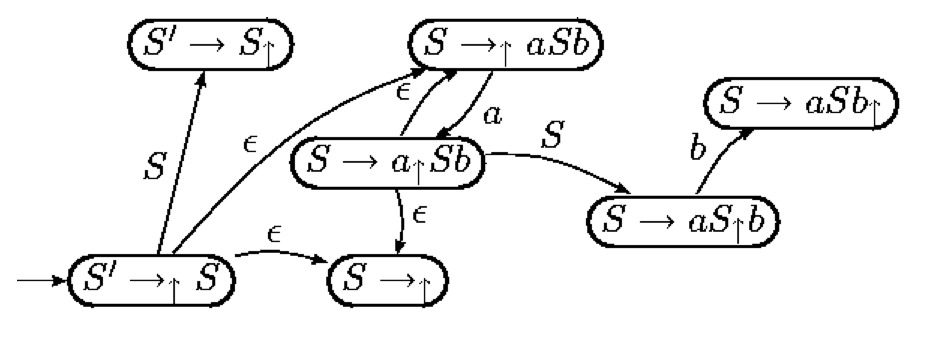
\epsfig{file=figures/nfa.eps, width=17cm}}
\caption{NFA que reconoce los prefijos viables}
\label{fig:nfa}
\end{figure}
%\end{makeimage}
\end{center}
\end{example}

\begin{exercise}
Simule el comportamiento del autómata sobre la entrada $aabb$. ¿Donde rechaza?
¿En que estados está el autómata en el momento del rechazo?. ¿Qué etiquetas tienen?
Haga también las
trazas del autómata para las entradas $aaSbb$ y $aSb$. ¿Que antiderivación 
ha construido el autómata con sus sucesivos rechazos? ¿Que terminales
se puede esperar que hayan en la entrada cuando se produce el rechazo
del autómata?
\end{exercise}

\section{Construcción de las Tablas para el Análisis SLR}

\subsection{Los conjuntos de Primeros y Siguientes}
Repasemos las nociones de conjuntos de \cei{Primeros} y \cei{siguientes}:

\begin{definition}
Dada una gramática $G=(\Sigma,V,P,S)$ y un símbolo $\alpha \in (V \cup \Sigma)^*$ se define el conjunto $FIRST(\alpha)$ como:

$FIRST(\alpha) = \left \{ b \in \Sigma :  \alpha  \stackrel{*}{\Longrightarrow}  b \beta \right \}
\cup N(\alpha)$ 

\noindent donde:

$N(\alpha) = \left \{ \begin{array}{ll}
                         \left \{ \epsilon \right \}& \mbox{si $\alpha \stackrel{*}{\Longrightarrow} \epsilon$} \\
                         \emptyset & \mbox{en otro caso} 
                      \end{array}
             \right. $ 

\end{definition}

\begin{definition}
Dada una gramática $G=(\Sigma,V,P,S)$ y una variable $A \in V$ se define el conjunto $FOLLOW(A)$ como: 

$FOLLOW(A) = \left \{ b \in \Sigma :  \exists\ S  \stackrel{*}{\Longrightarrow}  \alpha A b \beta \right \} \cup E(A)$

\noindent donde

$E(A) = \left \{ \begin{array}{ll}
                         \{ \$  \}& \mbox{si $S \stackrel{*}{\Longrightarrow} \alpha A$} \\
                         \emptyset & \mbox{en otro caso} 
                      \end{array}
             \right. $ 

\end{definition}

\begin{algorithm} Construcción de los conjuntos $FIRST(X)$
\begin{enumerate}
\item
$Si\ X \in \Sigma\ entonces\ FIRST(X) = {X}$
\item
$Si\ X \rightarrow \epsilon\ entonces\ FIRST(X) =  FIRST(X) \cup \{ \epsilon \}$
\item
$Si X \in V \ y\ X \rightarrow Y_1 Y_2 \cdots Y_k \in P\ entonces$
\begin{eqnarray*}
&&i = 1; \\
&&do\\
&&\ \ FIRST(X) = FIRST(X) \cup FIRST(Y_i) - \{ \epsilon \};\\
&&\ \ i++;\\
&&mientras\ (\epsilon \in FIRST(Y_i)\ and\ (i \leq k))\\
&&si\ (\epsilon \in FIRST(Y_k)\ and\ i > k)\ FIRST(X) = FIRST(X) \cup \{ \epsilon \}
\end{eqnarray*}
\end{enumerate}
\end{algorithm}
Este algoritmo puede ser extendido para calcular $FIRST(\alpha)$ para $\alpha = X_1 X_2 \cdots X_n \in (V \cup \Sigma)^*$.

\begin{algorithm} Construcción del conjunto $FIRST(\alpha)$ 
\begin{eqnarray*}
&&i = 1; \nonumber\\
&&FIRST(\alpha) = \emptyset; \nonumber\\
&&do \nonumber\\
&&\ \ FIRST(\alpha) = FIRST(\alpha) \cup FIRST(X_i) - \{ \epsilon \}; \nonumber\\
&&\ \ i++; \nonumber\\
&&mientras\ (\epsilon \in FIRST(X_i)\ and\ (i \leq n)) \nonumber\\
&&si\ (\epsilon \in FIRST(X_n)\ and\ i > n)\ FIRST(\alpha) = FIRST(X) \cup \{ \epsilon \}
\end{eqnarray*}
\end{algorithm} 

\begin{algorithm} Construcción de los conjuntos $FOLLOW(A)$
para las variables sintácticas $A \in V$: 

Repetir los siguientes pasos hasta que ninguno de los conjuntos $FOLLOW$ cambie:
\begin{enumerate} 
\item 
$FOLLOW(S) = \{\$\} $  ($\$$ representa el final de la entrada)
\item
$Si\ A \rightarrow \alpha B \beta\ entonces$
\[ FOLLOW(B) =  FOLLOW(B) \cup (FIRST(\beta) - \{\epsilon\})\]
\item
$Si\ A \rightarrow \alpha B$ o bien $A \rightarrow \alpha B \beta$
y $\epsilon \in FIRST(\beta)$  entonces

\[ FOLLOW(B) = FOLLOW(B) \cup FOLLOW(A)\]
\end{enumerate}
\end{algorithm}

\subsection{Construcción de las Tablas}
\label{subsection:nfa2dfa}

Para la construcción de las tablas de un analizador SLR
se construye el \cei{autómata finito determinista} (\cei{DFA}) 
$(Q, \Sigma, \delta, q_0)$ equivalente al NFA 
presentado en la sección
\ref{section:conceptosbasicos}
usando el \cei{algoritmo de construcción del subconjunto}.

Como recordará, en la construcción del subconjunto,
partiendo del estado de arranque $q_0$ del NFA con $\epsilon$-transiciones
se calcula su \cei{clausura} $\overline{\{q_0\}}$ y las 
clausuras de los conjuntos de estados $\overline{\delta(\overline{\{q_0\}},a)}$ 
a los que transita.  Se repite el proceso
con los conjuntos resultantes hasta que no se introducen nuevos
conjuntos-estado.

La clausura $\overline{A}$ de un subconjunto de estados del autómata $A$ esta formada
por todos los estados que pueden ser alcanzados mediante transiciones
etiquetadas con la palabra vacía (denominadas $\epsilon$ transiciones)
desde los estados de $A$. Se incluyen en $\overline{A}$, naturalmente los estados 
de $A$.

\begin{center}
$\overline{A} = \{ q \in Q\ /\  \exists q' \in Q\ :\ \hat{\delta}(q, \epsilon) = q \}$
\end{center}

Aquí $\hat{\delta}$ denota la \cei{función de transición del autómata} extendida  a cadenas
de $\Sigma^*$.

\begin{equation}
\label{equation:deltahat}
\hat{\delta}(q, x) = \left \{ \begin{array}{ll}
                         \delta(\hat{\delta}(q,y),a) & \mbox{si $x = ya$} \\
                         q & \mbox{si $x = \epsilon$} 
                      \end{array}
             \right.  
\end{equation}

En la práctica, y a partir de ahora así lo haremos, se prescinde de diferenciar
entre $\delta$ y $\hat{\delta}$ usándose indistintamente la notación
$\delta$ para ambas funciones.

La clausura puede ser computada usando una estructura de pila o aplicando 
la expresión recursiva dada en la ecuación \ref{equation:deltahat}.

Para el NFA mostrado en el ejemplo \ref{example:asb} el DFA construído mediante esta
técnica es el que se muestra en la figura \ref{fig:dfa}. Se ha utilizado el símbolo
\verb|#| como marcador. Se ha omitido el número 3 para que los estados coincidan
en numeración con los generados por \verb|yapp| (véase el cuadro
\ref{table:tablaslalr}).

\begin{center}
\begin{figure}
%\centerline{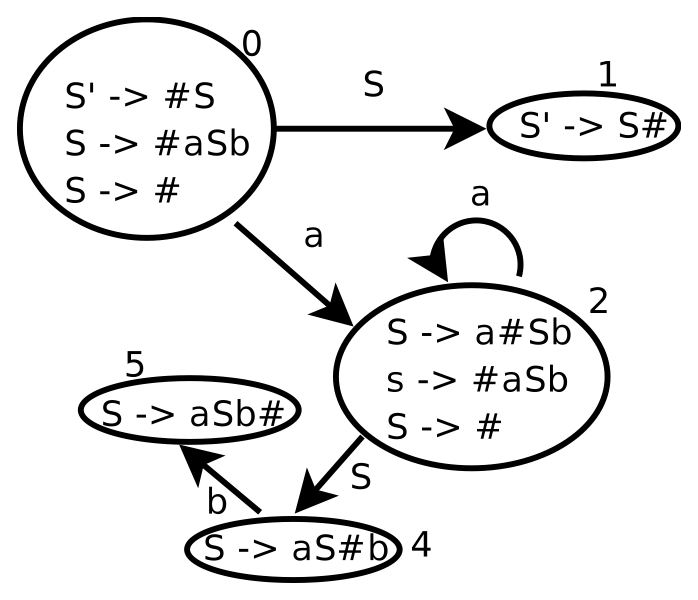
\epsfig{file=figures/dfa.eps, width=12cm}}
\caption{DFA equivalente al NFA de la figura \ref{fig:nfa}}
\label{fig:dfa}
\end{figure}
\end{center}

Un analizador sintáctico LR utiliza una tabla para su análisis.
Esa tabla se construye a partir de la tabla de transiciones del DFA.
De hecho, la tabla se divide en dos tablas, una llamada 
\cei{tabla de saltos} o \cei{tabla de gotos} y la otra
\cei{tabla de acciones}.

La tabla \cei{goto} de un analizador \cei{SLR}
no es más que la tabla de transiciones del autómata DFA 
obtenido aplicando la construcción del subconjunto al NFA
definido en \ref{definition:slrautomata}. De hecho es la tabla
de transiciones restringida a $V$ (recuerde que el alfabeto del
autómata es $V \cup \Sigma$).
Esto es, 

\begin{center}
$\delta_{| V \times Q} :  V \times Q \rightarrow Q$. 

donde se define $goto(i, A) = \delta(A,I_i)$
\end{center}

La parte de la función de transiciones
del DFA que corresponde a los terminales que no producen rechazo, 
esto es, $\delta_{| \Sigma \times Q} :  \Sigma \times Q \rightarrow Q$
se adjunta a una tabla que se denomina \cei{tabla de acciones}.
La tabla de acciones es una tabla de doble entrada en los estados
y en los símbolos de $\Sigma$.
Las acciones de transición ante terminales 
se denominan \cei{acciones de desplazamiento} o (\cei{acciones shift}):

\begin{center}
$\delta_{| \Sigma \times Q} :  \Sigma \times Q \rightarrow Q$

donde se define $action(i, a) = \delta(a,I_i)$
\end{center}

Cuando un estado $s$ contiene un LR(0)-item de la forma 
$A \rightarrow \alpha_\uparrow$, 
esto es, el estado corresponde a un posible rechazo,
ello indica que hemos llegado a un final del prefijo viable, que hemos
visto $\alpha$ y que, por tanto, es probable que $A \rightarrow \alpha$
sea el \emph{handle} de la forma sentencial derecha actual. Por tanto,
añadiremos en entradas de la forma $(s,a)$ de la tabla de acciones 
una acción que indique que hemos encontrado el mango en la 
posición actual y que la regla asociada es $A \rightarrow \alpha$.
A una acción de este tipo se la denomina \cei{acción de reducción}.

La cuestión es, ¿para que valores de $a \in \Sigma$ debemos disponer que
la acción para $(s, a)$ es de reducción?
Podríamos decidir que ante cualquier terminal $a \in \Sigma$
que produzca un rechazo del autómata, pero podemos ser un poco mas
selectivos. No cualquier terminal puede estar en la entrada en el momento
en el que se produce la antiderivación o reducción. 
Observemos que si $A \rightarrow \alpha$ es el \emph{handle}
de $\gamma$ es porque:

\begin{center}
$\exists S \begin{array}{c} *\\ \Longrightarrow \\ {\scriptstyle RM} \end{array} \beta A b x \begin{array}{c} *\\ \Longrightarrow \\ {\scriptstyle RM} \end{array}  
\beta \alpha b x = \gamma$
\end{center}

Por tanto, cuando estamos reduciendo por $A \rightarrow \alpha$
los únicos terminales legales que cabe esperar en una reducción por $A \rightarrow \alpha$ son los terminales $b \in FOLLOW(A)$.


Dada una gramática $G=(\Sigma,V,P,S)$, podemos construir las tablas de acciones (\emph{action table}) y  transiciones (\emph{gotos table}) mediante el siguiente algoritmo:

\begin{algorithm} 
\label{alg:tables}       
Construcción de Tablas \cei{SLR}

\begin{enumerate}
\item
Utilizando el Algoritmo de Construcción del Subconjunto, se construye
el Autómata Finito Determinista (DFA) $(Q, V \cup \Sigma, \delta, I_0, F)$
equivalente al Autómata Finito No
Determinista (NFA) definido en \ref{definition:slrautomata}.
Sea $C = \left \{ I_1, I_2, \cdots I_n \right \}$ el conjunto de estados
del DFA. Cada estado $I_i$ es un conjunto de LR(0)-items o estados
del NFA. Asociemos un índice $i$ con cada conjunto $I_i$.
\item
La tabla de \emph{gotos} no es más que la función de transición del 
autómata restringida a las variables de la gramática:

\begin{center}
$goto(i,A) = \delta(I_i, A)$ para todo $A \in V$
\end{center}
\item
Las acciones para el estado $I_i$ se determinan como sigue:
  \begin{enumerate}
  \item
  Si $A \rightarrow \alpha _\uparrow a \beta \in I_i$, $\delta(I_i,a) = I_j$, $a \in \Sigma$ 
  entonces:

\begin{center}
  $action[i][a] = shift\ j$
\end{center}
  \item
  Si $S' \rightarrow S_\uparrow \in I_i$ entonces 

\begin{center}
  $action[i][\$] = accept$
\end{center}
  \item
  Para cualquier otro caso de la forma $A \rightarrow \alpha _\uparrow \in I_i$ 
  distinto del anterior hacer

\begin{center}
  $\forall a \in\ FOLLOW(A):\ action[i][a] = reduce\ A \rightarrow \alpha$
\end{center}
  \end{enumerate}
\item
  Las entradas de la tabla de acción que queden indefinidas después de aplicado el proceso anterior corresponden a acciones de ``$error$''.
\end{enumerate}
\end{algorithm}

\begin{definition}
Si alguna de las entradas de la tabla resulta multievaluada, decimos
que existe un conflicto y que la gramática no es \cei{SLR}.

\begin{enumerate}
\item
En tal caso, si una de las acciones es de `reducción'' y la otra es de
`desplazamiento'', decimos que hay un \cei{conflicto shift-reduce} o
\cei{conflicto de desplazamiento-reducción}. 
\item
Si las
dos reglas indican una acción de reducción, decimos que tenemos un 
\cei{conflicto reduce-reduce} o de \cei{reducción-reducción}.
\end{enumerate}
\end{definition}

\begin{example}
\label{example:tablasslr}
Al aplicar el algoritmo \ref{alg:tables}       
a la gramática \ref{example:asb} 

\vspace{0.5cm}
\begin{center}
\begin{tabular}{|l|l|}
\hline
1 & S      $\rightarrow$  a S b\\
\hline
2 & S      $\rightarrow$ $\epsilon$ \\
\hline
\end{tabular}
\end{center}
\vspace{0.25cm}

partiendo del autómata finito determinista
que se construyó en 
la figura \ref{fig:dfa} y calculando los 
conjuntos de primeros y siguientes

\begin{center}
\begin{tabular}{|l|l|l|}
\hline
     & FIRST  & FOLLOW \\
\hline
S    & a, $\epsilon$ & b, \$\\
\hline
\end{tabular}
\end{center}

obtenemos la siguiente tabla de acciones SLR:

\begin{center}
\begin{tabular}{|l|l|l|l|}
\hline
     &  a  &  b  & \$ \\
\hline
0    & s2  &  r2 & r2 \\
\hline
1    &     &     & aceptar\\
\hline
2    & s2  & r2  & r2\\
\hline
4    &     & s5  &   \\
\hline
5    &     & r1  & r1\\
\hline
\end{tabular}
\end{center}

Las entradas denotadas con $s$ $n$ ($s$ por shift) indican un desplazamiento
al estado $n$, las denotadas con $r$ $n$ ($r$ por reduce o reducción) indican una operación
de reducción o antiderivación por la regla $n$.  Las entradas vacías 
corresponden a acciones de error.
\end{example}

El método de análisis \cei{LALR} usado por \verb|yapp|
es una extensión del método SLR esbozado
aqui. Supone un compromiso entre potencia (conjunto de gramáticas
englobadas) y eficiencia (cantidad de memoria utilizada, tiempo de
proceso).
Veamos como \verb|yapp| aplica la construcción del subconjunto a la 
gramática del ejemplo
\ref{example:asb}.
Para ello construimos el siguiente programa \verb|yapp|:
\begin{verbatim}
$ cat -n aSb.yp
     1  %%
     2  S:  # empty
     3      |   'a' S 'b'  
     4  ;
     5  %%
     ......
\end{verbatim}
y compilamos, haciendo uso de la opción \verb|-v| para que \verb|yapp| produzca
las tablas en el fichero \verb|aSb.output|:
\begin{verbatim}
$ ls -l aSb.*
-rw-r--r--  1 lhp lhp  738 2004-12-19 09:52 aSb.output
-rw-r--r--  1 lhp lhp 1841 2004-12-19 09:52 aSb.pm
-rw-r--r--  1 lhp lhp  677 2004-12-19 09:46 aSb.yp
\end{verbatim}

El contenido del fichero \verb|aSb.output| se muestra
en la tabla 
\ref{table:tablaslalr}.
Los números de referencia a las producciones en las acciones
de reducción vienen dados por:

\begin{verbatim}
                      0:	$start -> S $end
                      1:	S -> /* empty */
                      2:	S -> 'a' S 'b'
\end{verbatim} 

Observe que el final de la entrada se denota 
por \verb|$end| y el marcador en un LR-item 
por un punto. Fíjese en el estado 2: 
En ese estado están también los items

\begin{center}
 \verb|S -> . 'a' S 'b'|
y \verb|S -> .|
\end{center}

sin embargo no se explicitan
por que se entiende que su pertenencia es
consecuencia directa de aplicar la operación 
de clausura. Los LR items cuyo marcador
no está al principio se denominan
\cei{items núcleo}. 

\vspace{0.5cm}
\begin{table}[htb]
\begin{center}
\begin{tabular}{|p{4cm}|p{4cm}|p{4cm}|}
\hline
Estado 0 & Estado 1 & Estado 2\\
\hline
\begin{verbatim}
	$start -> . S $end	
	'a'	shift 2
	$default	reduce 1 (S)
	S	go to state 1
\end{verbatim} 
&
\begin{verbatim}
	$start -> S . $end	
	$end	shift 3
\end{verbatim} 
&
\begin{verbatim}
	S -> 'a' . S 'b'	
	'a'	shift 2
	$default	reduce 1 (S)
	S	go to state 4
\end{verbatim} 

\\

\hline
Estado 3 & Estado 4 & Estado 5\\
\hline

\begin{verbatim}
	$start -> S $end .	
	$default	accept
\end{verbatim} 
&
\begin{verbatim}
	S -> 'a' S . 'b'	
	'b'	shift 5
\end{verbatim} 
&
\begin{verbatim}
	S -> 'a' S 'b' .	
	$default	reduce 2 (S)
\end{verbatim}
\\
\hline
\end{tabular}
\end{center}
\caption{Tablas generadas por {\tt yapp}. El estado 3 resulta de transitar con \$}
\label{table:tablaslalr}
\end{table}
Puede encontrar el listado completo de las tablas en \verb|aSb.output|
en el apéndice que se encuentra en la página 
\ref{apendice:asb}.

\begin{exercise}
Compare la tabla \ref{table:tablaslalr} resultante de 
aplicar \verb|yapp| con la que obtuvo en el ejemplo
\ref{example:tablasslr}.
\end{exercise}

\section{El módulo Generado por {\tt yapp}}
\label{section:tablas}
La ejecución de la orden \verb|yapp -m Calc Calc.yp| produce 
como salida el módulo \verb|Calc.pm| el cual contiene las tablas LALR(1)
para la gramática descrita en \verb|Calc.yp|. Estas tablas son las que
dirigen al analizador LR. 
Puede ver el código completo del módulo en el apéndice
que se encuentra en la página \pageref{apendice:calcpm}.
La  estructura del módulo \verb|Calc.pm| es como sigue:

\begin{verbatim}
 1 package Calc;
 2 use vars qw ( @ISA );
 3 use strict;
 4 @ISA= qw ( Parse::Yapp::Driver );
 5 use Parse::Yapp::Driver;
 6 
 7 sub new {
 8    my($class)=shift;
 9    ref($class) and $class=ref($class);
10 
11     my($self)=$class->SUPER::new( 
12        yyversion => '1.05',
13        yystates => [ 
..          ...
32        ], # estados
33        yyrules  => [
..       	# ... mas reglas
70        ], # final de las reglas
71        @_); # argumentos pasados
72   bless($self,$class);
73 }
\end{verbatim}

La clase \verb|Calc| hereda de \verb|Parse::Yapp::Driver|, pero el objeto creado
será bendecido en la clase \verb|Calc| (Línea 4, véanse también 
la figura \ref{fig:yappinheritance} 
y la línea 72 del fuente). 
Por tanto, el constructor llamado en la línea 11 es el de \verb|Parse::Yapp::Driver|.
Se utiliza la estrategia de llamada con parámetros con nombre. 
El valor para la clave \verb|yystates| es una referencia anónima 
al array de estados y el valor para la clave \verb|yyrules| 
es una referencia anónima a las reglas.
\begin{verbatim}
10 
11     my($self)=$class->SUPER::new( 
12        yyversion => '1.05',
13        yystates => [
14         {#State 0
15           DEFAULT => -1, GOTOS => { 'input' => 1 }
16         },
17         {#State 1
18           ACTIONS => {
19             'NUM' => 6, '' => 4, "-" => 2, "(" => 7,
20             'VAR' => 8, "\n" => 5, 'error' => 9
21           },
22           GOTOS => { 'exp' => 3, 'line' => 10 }
23         },
24         # ...  mas estados
25         {#State 27
26           ACTIONS => {
27             "-" => 12, "+" => 13, "/" => 15, "^" => 16,
28             "*" => 17
29           },
30           DEFAULT => -8
31         }
32        ], # estados
\end{verbatim}
Se ve que un estado se pasa como un hash anónimo indexado en las acciones
y los saltos. 

Para consultar los números asociados con las reglas de producción
vea el apéndice en la página \pageref{apendice:calcouput}
conteniendo el fichero \verb|Calc.output|.

A continuación vienen las reglas:
\begin{verbatim}
33        yyrules  => [
34        [#Rule 0
35              '$start', 2, undef ],
36        [#Rule 1
37              'input', 0, undef ],
38        [#Rule 2
39              'input', 2, sub
40 #line 17 "Calc.yp"
41              { push(@{$_[1]},$_[2]); $_[1] }
42        ],
43        [#Rule 3
44              'line', 1, sub
45 #line 20 "Calc.yp"
46              { $_[1] }
47        ],
48        [#Rule 4
49              'line', 2, sub
50 #line 21 "Calc.yp"
51              { print "$_[1]\n" }
52        ],
53   # ... mas reglas
54     [#Rule 11
55             'exp', 3, sub
56 #line 30 "Calc.yp"
57 { $_[1] * $_[3] }
58    ],
59   [#Rule 12
60             'exp', 3, sub
61 #line 31 "Calc.yp"
62   {
63     $_[3] and return($_[1] / $_[3]);
64     $_[0]->YYData->{ERRMSG} =   "Illegal division by zero.\n";
65     $_[0]->YYError;
66     undef
67   }
68     ],
69   # ... mas reglas
70   ], # final de las reglas
\end{verbatim}
Las reglas son arrays anónimos conteniendo el nombre de la regla o
variable sintáctica (\verb|exp|), el número de símbolos en la parte
derecha y la subrutina anónima con el código asociado.

Vemos como la acción es convertida en una subrutina anónima. 
Los argumentos de dicha subrutina son los atributos semánticos
asociados con los símbolos en la parte derecha de la regla de 
producción. El valor retornado por la acción/subrutina
es el valor asociado con la reducción.

Para hacer que 
el compilador Perl diagnostique los errores relativos al fuente 
\verb|Calc.yp| se usa una directiva \verb|#line|.


\begin{verbatim}
71   @_);
72   bless($self,$class);
73 }
74 
\end{verbatim}

la bendición con dos argumentos hace que el objeto pertenezca a la
clase \verb|Calc|. A continuación siguen las subrutinas de soporte:
\begin{verbatim}
75 #line 44 "Calc.yp" 
76 
77 
78 sub _Error {
79   # ...
80 }
81 
82 sub _Lexer {
83   my($parser)=shift;
84   # ...
85 }
86 
87 sub Run {
88     my($self)=shift;
89     $self->YYParse( yylex => \&_Lexer, yyerror => \&_Error );
90 }
91 
92 my($calc)=new Calc;
93 $calc->Run;
94 
95 1;
\end{verbatim}

\section{Algoritmo de Análisis LR}
\label{section:algoritmoLR}
Asi  pues la tabla de transiciones del autómata nos genera dos tablas:
la tabla de acciones y la de saltos.
El  algoritmo  de análisis sintáctico \emph{LR} en el  que 
se basa \emph{yapp} utiliza una pila y dos tablas 
para analizar la entrada. % (véase la figura \ref{fig:lrparser}). 
Como se ha visto, la tabla  de acciones contiene cuatro tipo de acciones: 
\begin{enumerate}
\item
Desplazar (\emph{shift})
\item
Reducir (\emph{reduce})
\item
Aceptar
\item
Error
\end{enumerate}
El algoritmo utiliza una pila en la que se guardan los estados
del autómata. De este modo se evita tener que ``comenzar'' 
el procesado de la forma sentencial derecha resultante
después de una reducción (antiderivación).
\begin{algorithm}
\label{alg:parser}       
Análizador LR
\begin{verbatim}
push(s0);
 b = yylex();
 for( ; ; ;) {
   s = top(0); a = b;
   switch (action[s][a]) {
     case "shift t" : 
       push(t); 
       b = yylex();
       break;
     case "reduce A ->alpha" : 
       eval(Sub{A -> alpha}->(top(|alpha|-1).attr, ... , top(0).attr)); 
       pop(|alpha|); 
       push(goto[top(0)][A]); 
       break;
     case "accept" : return (1); 
     default : yyerror("syntax error");
   }
 }
\end{verbatim}
\end{algorithm}
Como es habitual, $|x|$ denota la longitud de la cadena $x$.
La función \verb|top(k)| devuelve el elemento que ocupa la 
posición \verb|k| desde el \emph{top} de la pila (esto es, está a profundidad \verb|k|).
La función \verb|pop(k)| extrae \verb|k| elementos de la pila.
La notación \verb|state.attr| hace referencia al atributo
asociado con cada estado. Denotamos por \verb|sub_{reduce A -> alpha}|
el código de la acción asociada con la regla $A \rightarrow \alpha$.
%\begin{figure}
%\input{parser_fig.tex}
%\caption{Estructura de un Análizador LR}
%\label{fig:lrparser}       
%\end{figure}

Todos los analizadores LR comparten, salvo pequeñas
exepciones, el mismo algoritmo
de análisis. Lo que más los diferencia es la forma en 
la que construyen las tablas.
En \verb|yapp|
la construcción de las tablas de \emph{acciones} y \emph{gotos}
se realiza mediante el algoritmo \emph{LALR}.

\section{Depuración en {\tt yapp}}
\label{section:depuracion}
Es posible añadir un parámetro en la llamada a \verb|YYParse|
con nombre \cei{yydebug} y valor el nivel de depuración requerido.
Ello 
nos permite observar la conducta del analizador. Los 
posibles valores de depuración son:

\vspace{0.5cm}
\begin{center}
\begin{tabular}{|l|l|}
\hline
   Bit      &    Información de Depuración \\
\hline
    0x01    &    Lectura de los terminales\\
\hline
    0x02    &    Información sobre los estados\\
\hline
    0x04    &    Acciones (shifts, reduces, accept \ldots)\\
\hline
    0x08    &    Volcado de la pila\\
\hline
    0x10    &    Recuperación de errores\\
\hline
\end{tabular}
\end{center}
\vspace{0.5cm}
 
 Veamos un ejemplo de salida para la gramática
 que se describe en la página 
 \pageref{apendice:asb}
 cuando se llama con: 

 \verb|$self->YYParse( yylex => \&_Lexer, yyerror => \&_Error, yydebug => 0x1F )|

 \begin{verbatim}
 1  $ ./use_aSb.pl
 2  ----------------------------------------
 3  In state 0:
 4  Stack:[0]
 5  ab  # el usuario ha escrito esto
 6  Need token. Got >a<
 7  Shift and go to state 2.
 8  ----------------------------------------
 9  In state 2:
10  Stack:[0,2]
11  Need token. Got >b<
12  Reduce using rule 1 (S,0): S -> epsilon
13  Back to state 2, then go to state 4.
14  ----------------------------------------
15  In state 4:
16  Stack:[0,2,4]
17  Shift and go to state 5.
18  ----------------------------------------
19  In state 5:
20  Stack:[0,2,4,5]
21  Don't need token.
22  Reduce using rule 2 (S,3): S -> a S b
23  Back to state 0, then go to state 1.
24  ----------------------------------------
25  In state 1:
26  Stack:[0,1]
27  Need token. Got ><
28  Shift and go to state 3.
29  ----------------------------------------
30  In state 3:
31  Stack:[0,1,3]
32  Don't need token.
33  Accept.
 \end{verbatim}

\section{Precedencia y Asociatividad}
\label{section:prioridades}
Recordemos que si al construir la tabla LALR,
alguna de las entradas de la tabla resulta multievaluada, decimos
que existe un conflicto.
Si una de las acciones es de `reducción'' y la otra es de
`desplazamiento'', se dice que hay un \cei{conflicto shift-reduce} o
\cei{conflicto de desplazamiento-reducción}. Si las
dos reglas indican una acción de reducción, decimos que tenemos un 
\cei{conflicto reduce-reduce} o de \cei{reducción-reducción}.
En caso de que no existan indicaciones específicas \emph{yapp} resuelve
los conflictos que aparecen en la construcción de la tabla utilizando
las siguientes reglas:

\begin{enumerate}
\item
Un conflicto \emph{reduce-reduce} se resuelve eligiendo la producción
que se listó primero en la especificación de la gramática.
\item
Un conflicto \emph{shift-reduce} se resuelve siempre en favor del \emph{shift}
\end{enumerate}

Las declaraciones de precedencia y asociatividad mediante las
palabras reservadas \tei{\%left}, \tei{\%right}, \tei{\%nonassoc}
se utilizan para modificar estos criterios por defecto. 
La declaración de \tei{token}s mediante la palabra
reservada \tei{\%token} no modifica la precedencia. Si lo hacen las
declaraciones realizadas usando las palabras \tei{left}, \tei{right}
y \tei{nonassoc}. 

\begin{enumerate}
\item
Los \emph{tokens} declarados  en la misma línea
tienen igual precedencia e igual asociatividad. 
La precedencia es mayor cuanto mas abajo 
su posición en
el texto. Así, en el ejemplo de la calculadora en la sección 
\ref{section:ejemplodeuso}, el \emph{token} \verb1*1 tiene 
mayor precedencia que \verb1+1 pero la misma que \verb1/1.
\item
La precedencia de una regla $A \rightarrow \alpha$ se
define como la del terminal mas a la derecha que aparece en
$\alpha$. En el ejemplo, la producción 

\begin{center}
\verb1 expr : expr '+' expr1 
\end{center}

tiene la precedencia del \emph{token} \verb1+1.
\item
Para decidir en un conflicto \emph{shift-reduce} se comparan la precedencia 
de la regla con la del terminal que va a ser desplazado. Si la de la
regla es mayor se reduce
si la del \emph{token} es mayor, se desplaza.
\item
Si en un conflicto \emph{shift-reduce} ambos la regla y el terminal que
va a ser desplazado tiene la misma precedencia \emph{yapp} considera la
asociatividad, si es asociativa a izquierdas, reduce y si es asociativa
a derechas desplaza. Si no es asociativa, genera un mensaje de error.\\
Obsérvese que, en esta situación, la asociatividad de la regla y la del
\emph{token} han de ser por fuerza, las mismas.  Ello es así, porque en
\emph{yapp} los \emph{tokens} con la misma precedencia se declaran en
la misma línea y sólo se permite una declaración por línea.

\item
\emph{ Por tanto es imposible declarar dos \emph{tokens} con diferente
asociatividad y la misma precedencia}.
\item
Es posible modificar la precedencia ``natural'' de una regla, calificándola
con un \emph{token} específico.  para ello se escribe a la derecha de
la regla \verb|prec token|, donde \verb|token| es un \emph{token} con
la precedencia que deseamos. Vea el uso del \emph{token} \verb|dummy|
en el siguiente ejercicio.
\end{enumerate}


Para ilustrar las reglas anteriores usaremos el siguiente 
programa \verb|yapp|:

\begin{verbatim}
$ cat -n Precedencia.yp
     1  %token NUMBER
     2  %left '@'
     3  %right '&'  dummy
     4  %%
     5  list
     6      :
     7      | list '\n'
     8      | list e
     9      ;
    10
    11  e : NUMBER
    12    | e '&' e
    13    | e '@' e %prec dummy
    14    ;
    15
    16  %%
\end{verbatim}            

El código del programa cliente es el siguiente:

\begin{verbatim}
$ cat -n useprecedencia.pl
cat -n useprecedencia.pl
     1  #!/usr/bin/perl -w
     2  use strict;
     3  use Precedencia;
     4
     5  sub Error {
     6    exists $_[0]->YYData->{ERRMSG}
     7    and do {
     8      print $_[0]->YYData->{ERRMSG};
     9      delete $_[0]->YYData->{ERRMSG};
    10      return;
    11    };
    12    print "Syntax error.\n";
    13  }
    14
    15  sub Lexer {
    16    my($parser)=shift;
    17
    18    defined($parser->YYData->{INPUT})
    19    or  $parser->YYData->{INPUT} = <STDIN>
    20    or  return('',undef);
    21
    22    $parser->YYData->{INPUT}=~s/^[ \t]//;
    23
    24    for ($parser->YYData->{INPUT}) {
    25        s/^([0-9]+(?:\.[0-9]+)?)//
    26                and return('NUMBER',$1);
    27        s/^(.)//s
    28                and return($1,$1);
    29    }
    30  }
    31
    32  my $debug_level = (@ARGV)? oct(shift @ARGV): 0x1F;
    33  my $parser = Precedencia->new();
    34  $parser->YYParse( yylex => \&Lexer, yyerror => \&Error, yydebug => $debug_level );
\end{verbatim}

Observe la llamada al analizador en la línea 34. Hemos 
añadido el parámetro con nombre \cei{yydebug} 
con argumento \verb|yydebug => $debug_level| (véase la
sección \ref{section:depuracion} para ver los posibles
valores de depuración).

Compilamos a continuación el módulo usando la opción \verb|-v| para
producir información sobre los conflictos y las tablas de salto y 
de acciones:
\begin{verbatim}
yapp -v -m Precedencia Precedencia.yp
$ ls -ltr |tail -2
-rw-r--r--  1 lhp lhp   1628 2004-12-07 13:21 Precedencia.pm
-rw-r--r--  1 lhp lhp   1785 2004-12-07 13:21 Precedencia.output
\end{verbatim}

La opción \verb|-v| genera el fichero \verb|Precedencia.output|
el cual contiene información detallada sobre el autómata:

\begin{verbatim}
$ cat -n Precedencia.output
     1  Conflicts:
     2  ----------
     3  Conflict in state 8 between rule 6 and token '@' resolved as reduce.
     4  Conflict in state 8 between rule 6 and token '&' resolved as shift.
     5  Conflict in state 9 between rule 5 and token '@' resolved as reduce.
     6  Conflict in state 9 between rule 5 and token '&' resolved as shift.
     7
     8  Rules:
     9  ------
    10  0:      $start -> list $end
    11  1:      list -> /* empty */
    12  2:      list -> list '\n'
    13  3:      list -> list e
    14  4:      e -> NUMBER
    15  5:      e -> e '&' e
    16  6:      e -> e '@' e
    17  ...
\end{verbatim}
¿Porqué se produce un conflicto en el estado 8 entre la regla
6 (\verb|e -> e '@' e|) y el terminal \verb|'@'|?. Editando el fichero
\verb|Precedencia.output| podemos ver los contenidos
del estado 8:
\begin{verbatim}
85  State 8:
86
87          e -> e . '&' e  (Rule 5)
88          e -> e . '@' e  (Rule 6)
89          e -> e '@' e .  (Rule 6)
90
91          '&'     shift, and go to state 7
92
93          $default        reduce using rule 6 (e)
\end{verbatim}
El item de la línea 88 indica que debemos desplazar, el de 
la línea 89 que debemos reducir por la regla 6. ¿Porqué \verb|yapp|
resuelve el conflicto optando por reducir?
¿Que prioridad tiene la regla 6?
¿Que asociatividad tiene la regla 6?
La declaración en la línea 13 modifica la precedencia y asociatividad
de la regla:

\begin{verbatim}
    13    | e '@' e %prec dummy
\end{verbatim}

de manera que la regla pasa a tener la precedencia y asociatividad
de \verb|dummy|. Recuerde que habíamos declarado \verb|dummy| como
asociativo a derechas:
\begin{verbatim}
     2  %left '@'
     3  %right '&'  dummy
\end{verbatim}
¿Que ocurre? Que \verb|dummy| tiene mayor prioridad
que \verb|'@'| y por tanto la regla tiene mayor prioridad
que el terminal: por tanto se reduce.

¿Que ocurre cuando el terminal en conflicto es \verb|'&'|?
En ese caso la regla y el terminal tienen la misma prioridad.
Se hace uso de la asociatividad a derechas que indica que el conflicto
debe resolverse desplazando.

\begin{exercise}
Explique la forma en que \verb|yapp| resuelve 
los conflictos que aparecen en el estado 9.
Esta es la información sobre el estado 9:

\begin{verbatim}
State 9:

	e -> e . '&' e	(Rule 5)
	e -> e '&' e .	(Rule 5)
	e -> e . '@' e	(Rule 6)
	'&'	shift, and go to state 7
	$default	reduce using rule 5 (e)
\end{verbatim}
\end{exercise}

Veamos un ejemplo de ejecución:

\begin{verbatim}
$ ./useprecedencia.pl
----------------------------------------
In state 0:
Stack:[0]
Don't need token.
Reduce using rule 1 (list,0): Back to state 0, then go to state 1.
\end{verbatim}
Lo primero que ocurre es una reducción por la regla 
en la que \verb|list| produce vacío. Si miramos el estado 0
del autómata vemos que contiene:
\begin{verbatim}
20 State 0:
21
22   $start -> . list $end (Rule 0)
23
24   $default  reduce using rule 1 (list)
25
26   list  go to state 1
\end{verbatim}
A continuación se transita desde 0 con \verb|list|
y se consume el primer terminal:
\begin{verbatim}
----------------------------------------
In state 1:
Stack:[0,1]
2@3@4
Need token. Got >NUMBER<
Shift and go to state 5.
----------------------------------------
In state 5:
Stack:[0,1,5]
Don't need token.
Reduce using rule 4 (e,1): Back to state 1, then go to state 2.
----------------------------------------
\end{verbatim}
En el estado 5 se reduce por la regla \verb|e -> NUMBER|.
Esto hace que se retire el estado 5 de la pila y se
transite desde el estado 1 viendo el símbolo \verb|e|:
\begin{verbatim}
In state 2:
Stack:[0,1,2]
Need token. Got >@<
Shift and go to state 6.
----------------------------------------
In state 6:
Stack:[0,1,2,6]
Need token. Got >NUMBER<
Shift and go to state 5.
----------------------------------------
In state 5:
Stack:[0,1,2,6,5]
Don't need token.
Reduce using rule 4 (e,1): Back to state 6, then go to state 8.
----------------------------------------
In state 8:
Stack:[0,1,2,6,8]
Need token. Got >@<
Reduce using rule 6 (e,3): Back to state 1, then go to state 2.
----------------------------------------
...
Accept.
\end{verbatim}
Obsérvese la resolución del conflicto en el estado 8

La presencia de conflictos, aunque no siempre, en muchos casos es debida
a la introducción de ambiguedad en la gramática. Si el conflicto 
es de desplazamiento-reducción se puede resolver explicitando 
alguna regla que rompa la ambiguedad. Los conflictos de
reducción-reducción suelen producirse por un diseño erróneo
de la gramática. En tales casos, suele ser mas adecuado
modificar la gramática.

\section{Generación interactiva de analizadores {\tt Yapp}}
En el siguiente código, la subrutina {\tt create\_yapp\_package} 
nos muestra como crear un analizador {\tt Yapp} en tiempo de ejecución.
Las dos líneas:
\begin{verbatim}
  my $p = new Parse::Yapp(input => $grammar);
  $p = $p->Output(classname => $name);
\end{verbatim}
crean una cadena en \verb|$p| conteniendo el código de 
la clase que implanta el analizador. Todo el truco está en hacer
\begin{verbatim}
  eval $p;
\end{verbatim}
para tener el paquete a mano:
\begin{verbatim}
$ cat left.pl
#!/usr/local/bin/perl5.8.0 -w
#use strict;
use Parse::Yapp;

sub lex{
    my($parser)=shift;

    return('',undef) unless $parser->YYData->{INPUT};
    for ($parser->YYData->{INPUT}) {
        s/^\s*//;
        s/^(.)//;
        my $ret = $1;
        return($ret, $ret);
    }
}

sub yapp {
  my $grammar = shift
     or die "Must specify a grammar as first argument";
  my $name = shift
     or die "Must specify the name of the class as second argument";

  my $p = new Parse::Yapp(input => $grammar) or die "Bad grammar.";
  $p = $p->Output(classname => $name) or die "Can't generate parser.";

  eval $p;
  $@ and die "Error while compiling your parser: $@\n";
}

######## main #########
my $grammar = q {
%left '*'
%%
S:  A
;

A:  A '*' A  { "($_[1] $_[2] $_[3])" }
 |  B
;

B:  'a' | 'b' | 'c' | 'd'
;

%%
};

&yapp($grammar, "Example");
my $p = new Example(yylex => \&lex, yyerror => sub {});

print "Expresion: ";
$p->YYData->{INPUT} = <>;
$p->YYData->{INPUT} =~ s/\s*$//;

my $out=$p->YYParse;
print "out = $out\n";
\end{verbatim}
Sigue un ejemplo de ejecución:
\begin{verbatim}
$ ./left.pl
Expresion: a*b*c*d
out = (((a * b) * c) * d)
\end{verbatim}

\section{Construcción del Árbol Sintáctico}
El siguiente ejemplo usa \verb|yapp| 
para construir el árbol sintáctico de una expresión en infijo:
\begin{verbatim}
$ cat -n Infixtree_bless.yp
 1  #
 2  # Infixtree.yp
 3  #
 4
 5  %{
 6  use Data::Dumper;
 7  %}
 8  %right  '='
 9  %left   '-' '+'
10  %left   '*' '/'
11  %left   NEG
12
13  %%
14  input:  #empty
15          |   input line
16  ;
17
18  line:     '\n'         { $_[1] }
19          | exp '\n'     { print Dumper($_[1]); }
20          | error '\n'   { $_[0]->YYErrok }
21  ;
22
23  exp:        NUM
24          |   VAR                 { $_[1] }
25          |   VAR '=' exp         { bless [$_[1], $_[3]], 'ASSIGN' }
26          |   exp '+' exp         { bless [$_[1], $_[3] ], 'PLUS'}
27          |   exp '-' exp         { bless [$_[1], $_[3] ], 'MINUS'}
28          |   exp '*' exp         { bless [$_[1], $_[3]], 'TIMES' }
29          |   exp '/' exp         { bless [$_[1], $_[3]], 'DIVIDE' }
30          |   '-' exp %prec NEG   { bless [$_[2]], 'NEG' }
31          |   '(' exp ')'         { $_[2] }
32  ;
33
34  %%
35
36  sub _Error {
37          exists $_[0]->YYData->{ERRMSG}
38      and do {
39          print $_[0]->YYData->{ERRMSG};
40          delete $_[0]->YYData->{ERRMSG};
41          return;
42      };
43      print "Syntax error.\n";
44  }
45
46  sub _Lexer {
47      my($parser)=shift;
48
49          defined($parser->YYData->{INPUT})
50      or  $parser->YYData->{INPUT} = <STDIN>
51      or  return('',undef);
52
53      $parser->YYData->{INPUT}=~s/^[ \t]//;
54
55      for ($parser->YYData->{INPUT}) {
56          s/^([0-9]+(?:\.[0-9]+)?)//
57                  and return('NUM',$1);
58          s/^([A-Za-z][A-Za-z0-9_]*)//
59                  and return('VAR',$1);
60          s/^(.)//s
61                  and return($1,$1);
62      }
63  }
64
65  sub Run {
66      my($self)=shift;
67      $self->YYParse( yylex => \&_Lexer, yyerror => \&_Error );
68  }
\end{verbatim}
Para compilar hacemos:
\begin{verbatim}
$ yapp -m Infixtree Infixtree_bless.yp
\end{verbatim}
El guión que usa el analizador anterior es similar al que vimos en la 
sección \ref{section:ejemplodeuso}:
\begin{verbatim}
$ cat -n ./useinfixtree.pl
     1  #!/usr/bin/perl -w
     2
     3  use Infixtree;
     4
     5  $parser = new Infixtree();
     6  $parser->Run;
\end{verbatim}
Veamos un ejemplo de ejecución:
\begin{verbatim}
$ ./useinfixtree.pl
a = 2+3
$VAR1 = bless( [
                 'a',
                 bless( [
                          '2',
                          '3'
                        ], 'PLUS' )
               ], 'ASSIGN' );
b = a*4+a
$VAR1 = bless( [
                 'b',
                 bless( [
                          bless( [
                                   'a',
                                   '4'
                                 ], 'TIMES' ),
                          'a'
                        ], 'PLUS' )
               ], 'ASSIGN' );
\end{verbatim}

\section{Acciones en Medio de una Regla}
A veces necesitamos insertar una acción en medio de una regla.
Una acción en medio de una regla puede hacer referencia a los atributos de
los símbolos que la preceden (usando \verb|$n|), pero no a los que le siguen.

Cuando se  inserta una acción $\left \{ action_1\right \}$
para su ejecución en medio de una regla $A \rightarrow \alpha
\beta$ :
\begin{center}
$A \rightarrow \alpha \left \{ action_1 \right \} \beta \left \{ action_2\right \}$ 
\end{center}
\verb|yapp| crea una variable sintáctica temporal $T$ e introduce una nueva regla:

\begin{center}
\begin{enumerate}
\item
$A \rightarrow \alpha T \beta \left \{ action_2\right \}$ 
\item
$T \rightarrow \epsilon \left \{ action_1 \right \}$ 
\end{enumerate}
\end{center}

Las acciones en mitad de una regla cuentan como un símbolo mas en la parte 
derecha de la regla. Asi pues, en una acción posterior en la regla,
se deberán referenciar los  atributos de los símbolos, teniendo en cuenta este hecho.

Las acciones en mitad de la regla pueden tener un atributo. 
Las acciones posteriores
en la regla se referirán a él como \verb|$_[n]|, siendo \verb|n| su número de orden
en la parte derecha. 

\section{Esquemas de Traducción}
Un \cei{esquema de traducción} es una gramática independiente del
contexto en la cuál se han asociado atributos a los símbolos de la gramática.
Un atributo queda caracterizado por un identificador
o nombre y un tipo o clase. Además se han insertado acciones, esto es,
código Perl/Python/C, \ldots en medio de las partes derechas.
En ese código es posible referenciar los atributos de los
símbolos de la gramática como variables del lenguaje subyacente.

Recuerde que el orden en que se evalúan los fragmentos de código
es el de un recorrido primero-profundo del árbol de análisis sintáctico.
Mas específicamente, considerando a las acciones como hijos-hoja del nodo,
el recorrido que realiza un esquema de traducción es:

\begin{verbatim}
 1     sub esquema_de_traduccion {
 2       my $node = shift;
 3 
 4       for my $child ($node->children) { # de izquierda a derecha
 5         if ($child->isa('ACTION') {
 6           $child->execute;
 7         }
 8         else { esquema_de_traduccion($child) }
 9       }
10     }
\end{verbatim}

Obsérvese que, como el bucle de la línea 4 recorre a los hijos
de izquierda a derecha, se debe dar la siguiente
condición para que un esquema  de traducción funcione:

Para cualquier regla de producción aumentada con acciones, de la forma 

\begin{center}
$A \rightarrow X_1 \ldots X_j$\verb|{ action($A{b}, $X|$_1$\verb|{c}|$ \ldots$\verb| X|$_n$\verb|{d})}|$X_{j+1} \ldots X_n$
\end{center}

debe ocurrir que los atributos evaluados en
la acción insertada después de $X_j$ 
dependan de atributos y variables que fueron computadas durante
la visita de los hermanos izquierdos o de sus ancestros.
En particular no deberían depender de atributos asociados
con las variables $X_{j+1} \ldots X_n$. Ello no significa que
no sea correcto evaluar atributos de $X_{j+1} \ldots X_n$
en esa acción.

\section{Definición Dirigida por la Sintáxis}
Una \cei{definición dirigida por la sintáxis} es un pariente cercano
de los esquemas de traducción. En una definición dirigida por la
sintáxis una gramática $G = (V, \Sigma, P, S)$ se aumenta 
con nuevas características:
\begin{itemize}
\item
A cada símbolo $S \in V \cup \Sigma$ de la gramática se le asocian
cero o mas atributos. Un atributo queda caracterizado por un identificador
o nombre y un tipo o clase. A este nivel son \cei{atributos formales},
como los parámetros formales, en el sentido de que su realización 
se produce cuando el nodo del árbol es creado.
\item
A cada regla de producción $A \rightarrow X_1 X_2 \ldots X_n \in P$
se le asocian un conjunto de \cei{reglas de evaluación de los atributos}
o \cei{reglas semánticas} que indican que el atributo en la parte
izquierda de la regla semántica depende de los atributos que aparecen en la parte
derecha de la regla. El atributo que aparece en la parte izquierda de la regla semántica
puede estar asociado con un símbolo en la parte derecha de la regla de producción.
\item
Los atributos de cada símbolo de la gramática $X \in V \cup \Sigma$
se dividen en dos grupos disjuntos: \cei{atributos sintetizados}
y \cei{atributos heredados}. Un atributo de $X$ es un \cei{atributo heredado} 
si depende de atributos de su padre y hermános en el árbol.
Un \cei{atributo sintetizado} es aquél tal que el valor del atributo depende
de los valores de los atributos de los hijos, 
es decir en tal caso $X$ ha de ser una variable sintáctica
y los atributos en la parte derecha de la regla semántica deben
ser atributos de símbolos en la parte derecha de la regla de producción 
asociada.
\item
Los atributos predefinidos se denominán \cei{atributos intrínsecos}.
Ejemplos de atributos intrínsecos son los atributos 
sintetizados de los terminales, los cuáles se han
computado durante la fase de análisis léxico. También
son atributos intrínsecos los atributos heredados del símbolo
de arranque, los cuales son pasados como parámetros 
al comienzo de la computación.
\end{itemize}

La diferencia principal con un esquema de traducción está en que
no se especifica el orden de ejecución de las reglas semánticas.
Se asume que, bien de forma manual o automática, se resolverán
las dependencias existentes entre los atributos determinadas
por la aplicación de las reglas semánticas, de manera
que serán evaluados primero aquellos atributos que no dependen
de ningún otro, despues los que dependen de estos, etc. siguiendo
un esquema de ejecución que viene guiado por las dependencias
existentes entre los datos.

Aunque hay muchas formas de realizar un evaluador de una definición
dirigida por la sintáxis, conceptualmente, tal evaluador debe:

\begin{enumerate}
\item
Construir el árbol de análisis sintáctico para la gramática
y la entrada dadas.
\item
Analizar las reglas semánticas para determinar los atributos,
su clase y las dependencias entre los mismos.
\item
Construir el \cei{grafo de dependencias} de los atributos,
el cual tiene
un nodo para cada ocurrencia de un atributo en el árbol de análisis
sintáctico etiquetado con dicho atributo. El grafo tiene una arista entre dos
nodos si existe una dependencia entre los dos atributos a través de alguna
regla semántica. 
\item
Supuesto que el grafo de dependencias determina un \cei{orden parcial}
(esto es cumple las propiedades reflexiva, antisimétrica y transitiva) 
construir un \cei{orden topológico} compatible con el orden parcial.
\item
Evaluar las reglas semánticas de acuerdo con el orden topológico.
\end{enumerate}

Una definición dirigida por la sintáxis en la que las reglas semánticas
no tienen efectos laterales se denomina una \cei{gramática atribuída}.

Si la definición dirigida por la sintáxis puede ser realizada 
mediante un esquema de traducción se dice que es \cei{L-atribuída}.
Para que una definición dirigida por la sintáxis sea L-atribuída
deben cumplirse que cualquiera que sea la regla de producción
$A \rightarrow X_1 \ldots X_n$, los atributos heredados de
$X_j$ pueden depender únicamente de:
\begin{enumerate}
\item
Los atributos de los símbolos a la izquierda de $X_j$
\item
Los atributos heredados de $A$
\end{enumerate}

Nótese que las restricciones se refieren a los atributos heredados.
El cálculo de los atributos sintetizados no supone 
problema para un esquema de traducción. Si la gramática
es LL(1), resulta fácil realizar una definición 
L-atribuída en un analizador descendente recursivo predictivo.

Si la definición dirigida por la sintáxis sólo utiliza 
atributos sintetizados se denomina \cei{S-atribuída}. Una
definición S-atribuída puede ser fácilmente trasladada a un programa
\verb|yapp|.

\section{Manejo en {\tt yapp} de Atributos Heredados}
\label{section:heredados}
Supongamos  que \verb|yapp| esta inmerso 
en la construcción de la antiderivación a derechas y que la forma sentencial
derecha en ese momento es:

\begin{center}
$X_m \ldots X_1 X_0 Y_1 \ldots  Y_n a_1 \ldots a_0$
\end{center}

y que el mango es $B \rightarrow Y_1 \ldots  Y_n$ y en la entrada quedan por 
procesar $a_1 \ldots a_0$.

Es posible acceder en \verb|yapp| a los valores de los atributos de los estados en la pila
del analizador que se encuentran ``por debajo'' o si se quiere
``a la izquierda'' de los estados asociados
con la regla por la que se reduce. Para ello se usa una llamada al método
\cei{{\tt YYSemval}}. La llamada es de la forma 
\verb|$_[0]->YYSemval( index )|, donde \verb|index| es un entero.
Cuando se usan los valores \verb|1| \ldots \verb|n| devuelve lo mismo
que \verb|$_[1]|, \ldots \verb|$_[n]|. Esto es 
\verb|$_[1]| es el atributo asociado con $Y_1$ y \verb|$_[n]| es el atributo
asociado con $Y_n$.  Cuando se usa con el valor
0 devolverá el valor del atributo asociado con el símbolo que esta a la izquierda 
del mango actual, esto es el atributo asociado con $X_0$, 
si se llama con -1 el que está dos unidades a la izquierda de la variable actual, 
esto es, el asociado con $X_1$ etc. Así \verb|$_[-m]| denota el atributo
de $X_m$.

Esta forma de acceder a los atributos es especialmente útil cuando se 
trabaja con \cei{atributos heredados}. Esto es, cuando un atributo
de un nodo del árbol sintáctico se computa en términos
de valores de atributos de su padre y/o sus hermanos.
Ejemplos de atributos heredados son la clase y tipo en la declaración
de variables. Supongamos que tenemos el siguiente 
\cei{esquema de traducción} para calcular la clase (C) y tipo (T) en 
las declaraciones (D) de listas (L) de identificadores:

\vspace{0.5cm}
\begin{center}
\begin{tabular}{|ll|}
\hline
D $\rightarrow$& C T \verb|{ $L{c} = $C{c}; $L{t} = $T{t} }| L\\
C $\rightarrow$& global   \verb|{ $C{c} = "global" }|\\
C $\rightarrow$& local    \verb|{ $C{c} = "local" }|\\
T $\rightarrow$& integer  \verb|{ $T{t} = "integer" }|\\
T $\rightarrow$& float    \verb|{ $T{t} = "float" }|\\
L $\rightarrow$& \verb|{ $L|$_1$\verb|{t} = $L{t}; $L|$_1$\verb|{c} = $L{c}; }| L$_1$ ','\\
               & id \verb|{ set_class($id{v}, $L{c}); set_type($id{v}, $L{t}); }|\\
L $\rightarrow$& id   \verb|{ set_class($id{v}, $L{c}); set_type($id{v}, $L{t}); }|\\
\hline
\end{tabular}
\end{center}
\vspace{0.25cm}

Los atributos \verb|c| y \verb|t| denotan respectivamente
la clase y el tipo. 

\begin{exercise}
Evalúe el esquema de traducción para la entrada
\verb|global float x,y|. Represente el árbol de análisis, las
acciones incrustadas y determine el orden de ejecución.

Olvide por un momento la notación usada en las acciones y 
suponga que se tratara de acciones \verb|yapp|. ¿En que orden
construye \verb|yapp| el árbol y en que orden ejecutará las
acciones?
\end{exercise}

A la hora de transformar este esquema de traducción en un programa
\verb|yapp| es importante darse cuenta que en cualquier derivación a derechas
desde D, cuando se reduce por una de las reglas 

\begin{center}
L $\rightarrow$ id $|$ L$_1$  ',' id
\end{center}

el símbolo a la izquierda de L es T y el que esta a la izquierda de T es C.
Considere, por ejemplo la derivación a derechas:

\begin{center}
D $\Longrightarrow$ C T L $\Longrightarrow$ C T L, id $\Longrightarrow$ C T L, id, id
$\Longrightarrow$ C T id, id, id $\Longrightarrow$ \\
$\Longrightarrow$ C float id, id, id $\Longrightarrow$ local float id, id, id
\end{center}

\noindent Observe que el orden de recorrido de \verb|yapp| es:
\begin{center}
local float id, id, id $\Longleftarrow$ C float id, id $\Longleftarrow$
C T id, id, id $\Longleftarrow$\\
$\Longleftarrow$ C T L, id, id $\Longleftarrow$ C T L, id $\Longleftarrow$ C T L $\Longleftarrow$ D
\end{center}

\noindent en la antiderivación, cuando el mango es una de las dos reglas 
para listas de identificadores, L $\rightarrow$ id y L $\rightarrow$ L, id 
es decir durante las tres ultimas antiderivaciones:

\begin{center}
C T L, id, id $\Longleftarrow$ C T L, id $\Longleftarrow$ C T L $\Longleftarrow$ D
\end{center}

\noindent las variables a la izquierda del mango son
T y C. Esto ocurre siempre. 
Estas observaciones nos conducen al siguiente
programa \verb|yapp|: 

\begin{verbatim}
$ cat -n Inherited.yp
 1  %token FLOAT INTEGER
 2  %token GLOBAL
 3  %token LOCAL
 4  %token NAME
 5
 6  %%
 7  declarationlist
 8    : # vacio
 9    | declaration ';' declarationlist
10    ;
11
12  declaration
13    : class type namelist { ; }
14    ;
15
16  class
17    : GLOBAL
18    | LOCAL
19    ;
20
21  type
22    : FLOAT
23    | INTEGER
24    ;
25
26  namelist
27    : NAME
28       { printf("%s de clase %s, tipo %s\n",
29               $_[1], $_[0]->YYSemval(-1),$_[0]->YYSemval(0)); }
30    | namelist ',' NAME
31        { printf("%s de clase %s, tipo %s\n",
32                 $_[3], $_[0]->YYSemval(-1),$_[0]->YYSemval(0)); }
33    ;
34  %%
\end{verbatim}

A continuación escribimos el programa que usa 
el módulo generado por \verb|yapp|:

\begin{verbatim}
$ cat -n useinherited.pl
 1  #!/usr/bin/perl -w
 2  use strict;
 3  use Inherited;
 4
 5  sub Error {
 6    exists $_[0]->YYData->{ERRMSG}
 7    and do {
 8      print $_[0]->YYData->{ERRMSG};
 9      delete $_[0]->YYData->{ERRMSG};
10      return;
11    };
12    print "Error sintáctico\n";
13  }
14
15  { # hagamos una clausura con la entrada
16    my $input;
17    local $/ = undef;
18    print "Entrada (En Unix, presione CTRL-D para terminar):\n";
19    $input = <stdin>;
20
21    sub scanner {
22
23      { # Con el redo del final hacemos un bucle "infinito"
24        if ($input =~ m|\G\s*INTEGER\b|igc) {
25          return ('INTEGER', 'INTEGER');
26        }
27        elsif ($input =~ m|\G\s*FLOAT\b|igc) {
28          return ('FLOAT', 'FLOAT');
29        }
30        elsif ($input =~ m|\G\s*LOCAL\b|igc) {
31          return ('LOCAL', 'LOCAL');
32        }
33        elsif ($input =~ m|\G\s*GLOBAL\b|igc) {
34          return ('GLOBAL', 'GLOBAL');
35        }
36        elsif ($input =~ m|\G\s*([a-z_]\w*)\b|igc) {
37          return ('NAME', $1);
38        }
39        elsif ($input =~ m/\G\s*([,;])/gc) {
40          return ($1, $1);
41        }
42        elsif ($input =~ m/\G\s*(.)/gc) {
43          die "Caracter invalido: $1\n";
44        }
45        else {
46          return ('', undef); # end of file
47        }
48        redo;
49      }
50    }
51  }
52
53  my $debug_level = (@ARGV)? oct(shift @ARGV): 0x1F;
54  my $parser = Inherited->new();
55  $parser->YYParse( yylex => \&scanner, yyerror => \&Error, yydebug => $debug_level );
\end{verbatim}
En las líneas de la 15 a la 51 esta nuestro analizador léxico.
La entrada se lee en una variable local cuyo valor permanece
entre llamadas: hemos creado una clausura con la variable
\verb|$input| (véase la sección \eref{section:clausura} para mas detalles
sobre el uso de clausuras en Perl). Aunque la variable \verb|$input|
queda inaccesible desde fuera de la clausura, persiste entre llamadas
como consecuencia de que la subrutina \verb|scanner| la utiliza.

A continuación sigue un ejemplo de ejecución:

\begin{verbatim}
$ ./useinherited.pl 0
Entrada (En Unix, presione CTRL-D para terminar):
global integer x, y, z;
local float a,b;
x de clase GLOBAL, tipo INTEGER
y de clase GLOBAL, tipo INTEGER
z de clase GLOBAL, tipo INTEGER
a de clase LOCAL, tipo FLOAT
b de clase LOCAL, tipo FLOAT
\end{verbatim}

\begin{exercise}
El siguiente programa \verb|yapp| calcula 
un árbol de análisis abstracto para la gramática
del ejemplo anterior:
\begin{verbatim}
%token FLOAT INTEGER 
%token GLOBAL 
%token LOCAL 
%token NAME

%%
declarationlist 
  : /* vacio */                     { bless [], 'declarationlist' } 
  | declaration ';' declarationlist { push @{$_[3]}, $_[1]; $_[3] }
  ;

declaration
  : class type namelist 
      { 
        bless {class => $_[1], type => $_[2], namelist => $_[3]}, 'declaration'; 
      }
  ;

class
  : GLOBAL  { bless { GLOBAL => 0}, 'class' } 
  | LOCAL   { bless { LOCAL => 1}, 'class' }
  ;

type
  : FLOAT   { bless { FLOAT => 2}, 'type' } 
  | INTEGER { bless { INTEGER => 3}, 'type' }
  ;

namelist
  : NAME  
     { bless [ $_[1]], 'namelist' }
  | namelist ',' NAME 
      { push @{$_[1]}, $_[3]; $_[1] }
  ;
%%
\end{verbatim}
sigue un ejemplo de ejecución:
\begin{verbatim}
$ ./useinherited3.pl
Entrada (En Unix, presione CTRL-D para terminar):
global float x,y;
$VAR1 = bless( [
  bless( {
    'namelist' => bless( [ 'x', 'y' ], 'namelist' ),
    'type' => bless( { 'FLOAT' => 2 }, 'type' ),
    'class' => bless( { 'GLOBAL' => 0 }, 'class' )
  }, 'declaration' )
], 'declarationlist' );
\end{verbatim}

Extienda el programa del ejemplo para que la gramática 
incluya las acciones del esquema de traducción.
Las acciones se tratarán como un terminal \verb|CODE|
y serán devueltas por el analizador léxico. Su atributo
asociado es el texto del código. El programa 
\verb|yapp| deberá devolver el árbol abstracto
extendido con las acciones-terminales.
La parte mas difícil de este problema consiste en ``reconocer''
el código Perl incrustado. La estrategia seguir consiste
en contar el número de llaves que se abren y se cierran.
Cuando el contador alcanza cero es que hemos llegado
al final del código Perl incrustado. Esta estrategia
tiene una serie de problemas. ¿Sabría decir cuáles?
(sugerencia: repase la sección \ref{subsection:elcuerpo} 
o vea como \verb|yapp| resuelve el problema).
\end{exercise}

\section{Acciones en Medio de una Regla y Atributos Heredados}
\label{section:mediaregla}
La estrategia utilizada en la sección \ref{section:heredados} funciona
si podemos predecir la posición del atributo en la pila del analizador.
En el ejemplo anterior los atributos clase y tipo estaban siempre,
cualquiera que fuera la derivación a derechas, 
en las posiciones 0 y -1. Esto no siempre es asi. Consideremos
la siguiente \cei{definición dirigida por la sintáxis}:

\vspace{0.5cm}
\begin{center}
\begin{tabular}{|l|l|}
\hline
S $\rightarrow$ a A C   & \verb|$C{i} = $A{s}|\\
\hline
S $\rightarrow$ b A B C & \verb|$C{i} = $A{s}|\\
\hline
C $\rightarrow$ c       & \verb|$C{s} = $C{i}|\\
\hline
A $\rightarrow$ a       & \verb|$A{s} = "a"|\\
\hline
B $\rightarrow$ b       & \verb|$B{s} = "b"|\\
\hline
\end{tabular}
\end{center}
\vspace{0.25cm}


\begin{exercise}
Determine un orden correcto de evaluación de la anterior
definición dirigida por la sintáxis para la entrada \verb|b a b c|.
\end{exercise}

C hereda el atributo sintetizado de A. El problema es que, en la pila
del analizador el atributo \verb|$A{s}| puede estar en la posición 0 
o -1 dependiendo de si la regla por la que se derivó fué
S $\rightarrow$ a A C o bien S $\rightarrow$ b A B C. La solución
a este tipo de problemas consiste en insertar acciones 
intermedias de copia del atributo de manera que se garantize que el atributo
de interés está siempre a una distancia fija. Esto es, se inserta
una variable sintáctica intermedia auxiliar M la cual deriva a vacío
y que tiene como acción asociada una regla de copia:

\vspace{0.5cm}
\begin{center}
\begin{tabular}{|l|l|}
\hline
S $\rightarrow$ a A C   & \verb|$C{i} = $A{s}|\\
\hline
S $\rightarrow$ b A B M C & \verb|$M{i} = $A{s}; $C{i} = $M{s}|\\
\hline
C $\rightarrow$ c       & \verb|$C{s} = $C{i}|\\
\hline
A $\rightarrow$ a       & \verb|$A{s} = "a"|\\
\hline
B $\rightarrow$ b       & \verb|$B{s} = "b"|\\
\hline
M $\rightarrow \epsilon$& \verb|$M{s} = $M{i}|\\
\hline
\end{tabular}
\end{center}
\vspace{0.25cm}

El nuevo esquema de traducción puede ser implantado mediante
un programa \verb|yapp|:

\begin{verbatim}
$ cat -n Inherited2.yp
     1  %%
     2  S : 'a' A C
     3    | 'b' A B  { $_[2]; } C
     4    ;
     5
     6  C : 'c' { print "Valor: ",$_[0]->YYSemval(0),"\n"; $_[0]->YYSemval(0) }
     7    ;
     8
     9  A : 'a' { 'a' }
    10    ;
    11
    12  B : 'b' { 'b' }
    13    ;
    14
    15  %%
\end{verbatim}

La ejecución muestra como se ha propagado el valor del atributo:
\begin{verbatim}
$ ./useinherited2.pl '0x04'
Entrada (En Unix, presione CTRL-D para terminar):
b a b c
Shift 2.  Shift 6.
Reduce using rule 5 (A,1): Back to state 2, then state 5.
Shift 8.
Reduce 6 (B,1): Back to state 5, then state 9.
Reduce 2 (@1-3,0): Back to state 9, then state 12.
\end{verbatim}

En este momento se esta ejecutando la acción intermedia.
Lo podemos comprobar revisando el fichero \verb|Inherited2.output|
que fué generado usando la opción \verb|-v| al llamar a \verb|yapp|.
La regla 2 por la que se reduce es la asociada con la acción 
intermedia:

\begin{verbatim}
$ cat -n Inherited2.output
     1  Rules:
     2  ------
     3  0:      $start -> S $end
     4  1:      S -> 'a' A C
     5  2:      @1-3 -> /* empty */
     6  3:      S -> 'b' A B @1-3 C
     7  4:      C -> 'c'
     8  5:      A -> 'a'
     9  6:      B -> 'b'
        ...
\end{verbatim}

Obsérvese la notación usada por \verb|yapp| para la 
\cei{acción en medio de la regla}: \verb|@1-3|.
Continuamos con la antiderivación:

\begin{verbatim}
Shift 10.
Reduce 4 (C,1): 
Valor: a
Back to state 12, then 13.
Reduce using rule 3 (S,5): Back to state 0, then state 1.
Shift 4.
Accept.
\end{verbatim}

El método puede ser generalizado a casos en los
que el atributo de interés este a diferentes distancias en
diferentes reglas sin mas que introducir las correspondientes
acciones intermedias de copia.

\section{Recuperación de Errores}
\label{section:errores}
Las entradas de un traductor pueden contener errores. 
El lenguaje \verb|yapp| proporciona un \emph{token} especial,
\verb|error|, que puede ser utilizado en el programa fuente
para extender el traductor con ``producciones de error'' 
que lo doten de cierta capacidad para 
recuperase de  una entrada errónea y poder continuar 
analizando el resto de la entrada.

Consideremos lo que ocurre al ejecutar nuestra calculadora
\verb|yapp| con una entrada errónea. Recordemos 
la gramática:

\begin{verbatim}
 9  %right  '='
10  %left   '-' '+'
11  %left   '*' '/'
12  %left   NEG
13  %right  '^'
14
15  %%
16  input:  # empty
17          |   input line  { push(@{$_[1]},$_[2]); $_[1] }
18  ;
19
20  line:       '\n'       { $_[1] }
21          |   exp '\n'   { print "$_[1]\n" }
22          |   error '\n' { $_[0]->YYErrok }
23  ;
\end{verbatim}

La regla \verb|line |$\rightarrow$ \verb|error '\n'| es una producción de
error. La idea general de uso es que, a traves de la misma, el programador 
le indica a \verb|yapp| que, cuando se produce un error
dentro de una expresión, descarte todos los \emph{tokens} hasta llegar al
retorno del carro y prosiga con el análisis. 
Además, mediante la llamada al método \verb|YYErrok| el programador
anuncia que, si se alcanza este punto, la recuperación puede considerarse 
``completa''  y que \verb|yapp| puede emitir a partir de ese momento 
mensajes de error
con la seguridad de que no son consecuencia de un comportamiento inestable
provocado por el primer error.

El resto de la gramática de la calculadora era como sigue:

\begin{verbatim}
24
25  exp:        NUM
26          |   VAR                 { $_[0]->YYData->{VARS}{$_[1]} }
27          |   VAR '=' exp         { $_[0]->YYData->{VARS}{$_[1]}=$_[3] }
28          |   exp '+' exp         { $_[1] + $_[3] }
29          |   exp '-' exp         { $_[1] - $_[3] }
30          |   exp '*' exp         { $_[1] * $_[3] }
31          |   exp '/' exp         {
32                                    $_[3]
33                                    and return($_[1] / $_[3]);
34                                    $_[0]->YYData->{ERRMSG}
35                                      =   "Illegal division by zero.\n";
36                                    $_[0]->YYError;
37                                    undef
38                                  }
39          |   '-' exp %prec NEG   { -$_[2] }
40          |   exp '^' exp         { $_[1] ** $_[3] }
41          |   '(' exp ')'         { $_[2] }
42  ;
\end{verbatim}
en la ejecución activamos el flag \verb|yydebug| a \verb|0x10| para 
obtener información sobre el tratamiento de errores:
\begin{verbatim}
$self->YYParse( yylex => \&_Lexer, yyerror => \&_Error, yydebug => 0x10 );
\end{verbatim}
Pasemos a darle una primera entrada errónea:

\begin{verbatim}
$ ./usecalc.pl
3-+2
Syntax error.
**Entering Error recovery.
**Pop state 12.
**Pop state 3.
**Shift $error token and go to state 9.
**Dicard invalid token >+<.
**Pop state 9.
**Shift $error token and go to state 9.
**Dicard invalid token >NUM<.
**Pop state 9.
**Shift $error token and go to state 9.
**End of Error recovery.
\end{verbatim}


El esquema general del algoritmo de recuperación de errores usado 
por la versión actual de \verb|yapp| es el siguiente:

\begin{enumerate}
\item
Cuando se encuentra ante una acción de error, el analizador genera un 
\emph{token} \verb1error1.

\item
A continuación pasa a retirar estados de la pila hasta que descubre un
estado capaz de transitar ante el \emph{token} \verb1error1. 
En el ejemplo anterior el analizador estaba en el estado 12 y lo retira
de la pila. Los contenidos del estado 12 son:
\begin{verbatim}
	exp -> exp '-' . exp	(Rule 10)
	'('	shift 7 '-'	shift 2 NUM	shift 6 VAR	shift 8
	exp	go to state 21
\end{verbatim}
Obviamente no esperabamos ver un \verb|'+'| aqui. El siguiente
estado en la cima de la pila es el 3, el cual tampoco
tiene ninguna transición ante el terminal \verb|error|:

\begin{verbatim}
	line -> exp . '\n'	(Rule 4)
	exp -> exp . '+' exp	(Rule 9)
	exp -> exp . '-' exp	(Rule 10)
	exp -> exp . '*' exp	(Rule 11)
	exp -> exp . '/' exp	(Rule 12)
	exp -> exp . '^' exp	(Rule 14)

	'*'	shift 17 '+'	shift 13 '-'	shift 12 '/'	shift 15
	'\n'	shift 14 '^'	shift 16
\end{verbatim}
El pop sobre el estado 3 deja expuesto en la superficie al estado
1, el cuál ``sabe'' como manejar el error:
\begin{verbatim}
	$start -> input . $end	(Rule 0)
	input -> input . line	(Rule 2)

	$end	shift 4 '('	shift 7 '-'	shift 2 '\n'	shift 5
	NUM	shift 6 VAR	shift 8
	error	shift 9

	exp	go to state 3
	line	go to state 10
\end{verbatim}

\item
En este punto transita al estado correspondiente a desplazar el 
\emph{token} \verb1error1. 

En consecuencia, con lo dicho, en el ejemplo se va al estado 9:
\begin{verbatim}
	line -> error . '\n'	(Rule 5)
	'\n'	shift, and go to state 20
\end{verbatim}

\item
Entonces el algoritmo de recuperación va
leyendo \emph{tokens} y descartandolos hasta encontrar
uno que sea aceptable. En este caso hemos especificado
que el terminal que nos da cierta confianza de recuperación
es el retorno de carro:
\begin{verbatim}
**Dicard invalid token >+<.
**Pop state 9.
**Shift $error token and go to state 9.
**Dicard invalid token >NUM<.
**Pop state 9.
**Shift $error token and go to state 9.
**End of Error recovery.
\end{verbatim}

\item
Sólo se envían nuevos mensajes de error una vez asimilados (desplazados)
algunos símbolos terminales. De este modos se intenta evitar la aparición
masiva de mensajes de error.
\end{enumerate}

\section{Recuperación de Errores en Listas}
Aunque no existe un método exacto para decidir como ubicar
las reglas de recuperación de errores, 
en general, los s\'{\i}mbolos de error deben ubicarse intentado 
satisfacer las siguientes reglas:

\begin{itemize}
\item
Tan cerca como sea posible del s\'{\i}mbolo de arranque.
\item
Tan cerca como sea posible de los s\'{\i}mbolos terminales.
\item
Sin introducir nuevos conflictos.
\end{itemize}

En el caso particular de las listas, se recomienda seguir el
siguiente esquema:

\vspace{0.5cm}
\begin{table}
\begin{center}
\begin{tabular}{|l|l|l|}
\hline
Construcción       & EBNF & yapp\\
\hline
secuencia opcional & x:\{y\}   & \verb#x : /* null */             #\\ 
                   &           & \verb#  | x y  { $_[0]->YYErrok; }      #\\
                   &           & \verb#  | x error                #\\
\hline
secuencia          & x:y\{y\}  & \verb#x : y                      #\\ 
                  &           & \verb#  | xy   { $_[0]->YYErrok; }      #\\
                &           & \verb#  | error                  #\\
                &           & \verb#  | x error                #\\
\hline
lista              & x:y\{Ty\} & \verb#x : y                       #\\ 
                  &           & \verb#  | x T y { $_[0]->YYErrok; }      #\\
                &           & \verb#  | error                   #\\
                &           & \verb#  | x error                 #\\
                &           & \verb#  | x error y { $_[0]->YYErrok; }  #\\
                &           & \verb#  | x  T error              #\\
\hline
\end{tabular}
\end{center}
\caption{Recuperación de errores en listas}
\label{table:err}
\end{table}
\vspace{0.25cm}

\begin{exercise} 
Compruebe el funcionamiento de la metodología 
para la recuperación de errores en listas presentada
en la tabla \ref{table:err}
estudie el siguiente programa \verb|yapp| siguiendo la traza de estados,
generando entradas con todos los tipos de error posibles.
¿Cómo se recupera el analizador en caso de existencia de un segundo
error? ¿Que ocurre si dos errores consecutivos 
están muy próximos?
El programa corresponde al tercer caso de la tabla \ref{table:err}, 
el caso x:y\{Ty\} con 
x = {\tt list}, T = {\tt ','} e y = {\tt NUMBER}:
\begin{verbatim}
%token NUMBER
%%
command 
  : 
  | command list '\n' { $_[0]->YYErrok; } 
  ;

list 
    : NUMBER            { put($1); }
    | list ',' NUMBER   { put($3); $_[0]->YYErrok; }
    | error             { err(1); }
    | list error        { err(2); }
    | list error NUMBER { err(3); put($3); $_[0]->YYErrok; }
    | list ',' error    { err(4); }
    ;
    
%%    
sub put { my $x = shift; printf("%2.1lf\n",$x); }
sub err { my $code = shift; printf("err %d\n",$code); }
 ...
\end{verbatim} 
\end{exercise} 

\section{Consejos a seguir al escribir un programa {\tt yapp}}
\label{section:consejosyapp}
Cuando escriba un programa \verb|yapp| asegurese
de seguir los siguientes consejos:

\begin{enumerate}
\item
Coloque el punto y coma de separación de reglas en una línea aparte.
Un punto y coma ``pegado'' al final de una regla puede confundirse
con un terminal de la regla.

\item
Si hay una regla que produce vacío, coloquela en primer lugar y acompáñela de 
un comentario resaltando ese hecho.
\item
Nunca escriba dos reglas de producción en la misma línea.
\item
Sangre convenientemente todas las partes derechas de las reglas
de producción de una variable, de modo que queden
alineadas.
\item
Ponga nombres representativos a sus variables sintácticas. No llame 
\verb|Z| a una variable que representa el concepto ``lista de parámetros'',
llámela \verb|ListaDeParametros|.
\item
Es conveniente que declare los terminales simbólicos, esto es, aquellos que 
llevan un identificador asociado. Si no llevan prioridad asociada o no 
es necesaria, use una declaración \verb|%token|. De esta manera
el lector de su programa se dará cuenta rápidamente que dichos identificadores
no se corresponden con variables sintácticas. Por la misma razón,
si se trata de terminales
asociados con caracteres o cadenas no es tan necesario que los declare, 
a menos que, 
como en el ejemplo de la calculadora para \verb|'+'| y \verb|'*'|,
sea necesario asociarles una
precedencia.
\item
Es importante que use la opción \verb|-v| para producir
el fichero \verb|.output| conteniendo información detallada sobre
los conflictos y el autómata. Cuando haya un conflicto shift-reduce
no resuelto busque en el fichero el estado implicado y 
vea que LR(0) items $A \rightarrow \alpha_\uparrow$
y $B \rightarrow \beta_\uparrow \gamma$ entran en conflicto.

\item
\label{item:conflictos}
Si según el informe de \verb|yapp|
el conflicto se produce ante un terminal $a$,
es porque $a \in FOLLOW(A)$ y
$a \in FIRST(\gamma)$. Busque las causas por las que esto ocurre 
y modifique su gramática con vistas a eliminar la presencia
del terminal $a$ en uno de los dos conjuntos implicados
o bien establezca reglas de prioridad entre los terminales
implicados que resuelvan el conflicto.

\item
Nótese que cuando existe un conflicto de desplazamiento 
reducción entre $A \rightarrow \alpha_\uparrow$ 
y  $B \rightarrow \beta_\uparrow \gamma$, el programa
\verb|yapp| contabiliza un error por cada terminal 
$a \in FOLLOW(A) \cap FIRST(\gamma)$. Por esta razón,
si hay 16 elementos en $FOLLOW(A) \cap FIRST(\gamma)$,
el analizador \verb|yapp| informará de la existencia
de 16 conflictos \emph{shift-reduce},
cuando en realidad se trata de uno sólo. No desespere, 
los conflictos ``auténticos'' suelen
ser menos de los que \verb|yapp| anuncia.

\item
Si necesita declarar variables globales, inicializaciones, etc.
que afectan la conducta global del analizador, escriba el código 
correspondiente en la cabecera del analizador, protegido
por los delimitadores \verb|%{| y \verb|%}|. Estos delimitadores
deberán aparecer en una línea aparte. Por ejemplo:

\begin{verbatim}
%{
our contador = 0;
%}

%token NUM
...
%%
\end{verbatim}

\item
Si tiene problemas en tiempo de ejecución con el comportamiento del análizador
sintáctico use la opción \verb|yydebug => 0x1F| en la llamada al analizador.

\item
Si trabaja en windows y pasa los ficheros a unix tenga cuidado con la posible
introducción de caractéres espúreos en el fichero. Debido
a la presencia de caractéres de control invisibles, el analizador \verb|yapp| 
pasará a rechazar una gramatica aparentemente correcta.

\item
Sea consciente de que los analizadores sintáctico y  léxico mantienen
una relación de corutinas en \verb|yapp|: Cada vez que 
el analizador sintáctico necesita un nuevo terminal para decidir que regla de
producción se aplica, llama al analizador léxico, el cuál deberá retornar el siguiente
terminal. La estrategia es diferente de la utilizada en el ejemplo
usado para el lenguaje Tutu en el capítulo 
\ref{chapter:introcomp}. Allí generabamos en una primera fase
la lista de terminales. Aquí los terminales se generan  de uno en uno
y cada vez que se encuentra uno nuevo se retorna al analizador sintáctico.
La ventaja que tiene este método es que permite colaborar al analizador sintáctico
y al analizador léxico para ``dinámicamente'' modificar la conducta 
del análisis léxico. Por ejemplo en los compiladores del lenguaje C
es común hacer que el analizador léxico cuando descubre un identificador que 
previamente ha sido declarado como identificador de tipo (mediante 
el uso de \verb|typedef|) retorne un terminal \verb|TYPENAME| 
diferente del terminal \verb|ID|
que caracteriza a los identificadores. Para ello, el analizador
sintáctico, cuando detecta una tal declaración, ``avisa'' al analizador 
léxico para que modifique su conducta. El analizador sintáctico volverá
a avisarlo cuando la declaración del identificador como
identificador de tipo salga de ámbito y pierda
su especial condición.  

\item
En \verb|yapp| el analizador sintáctico espera que el analizador
léxico devuelva de cada vez una pareja formada por dos escalares.
El primer escalar es la cadena que designa el terminal. A diferencia
de la habitual costumbre \verb|yacc| de codificar los terminales
como enteros, en \verb|yapp| se suelen codificar como cadenas.
La segunda componente de la pareja es el atributo asociado con el terminal.
Si el atributo es un atributo complejo que necesitas representar
mediante un hash o un vector, lo mejor es hacer que esta componente
sea una referencia al objeto describiendo el atributo.
El analizador léxico le indica al sintáctico la
finalización de la entrada enviándole la pareja 
\verb|('',undef)| formada por la palabra vacía con atributo \verb|undef|.

\item
Hay fundamentalmente dos formas de hacer el analizador
léxico: hacerlo destructivo o no destructivo.
En los destructivos se usa el operador de sustitución \verb|s|
(véase el ejemplo de la sección 
\ref{section:ejemplodeuso}), en cuyo caso la entrada procesada
es retirada de la cadena leída.
En los no destructivos utilizamos el operador
de emparejamiento \verb|m|. Véase 
el ejemplo de analizador léxico en
la sección \ref{section:heredados}
(concretamente la subrutina \verb|scanner| en la 
línea 20 del fichero \verb|useinherited.pl|)
\end{enumerate}

\begin{example}
Consideremos de nuevo el programa \verb|yapp| para producir
árboles para las expresiones en infijo. Supongamos que olvidamos
introducir una prioridad explícita al terminal \verb|'='|:
\begin{verbatim}
$ cat -n Infixtree_conflict.yp
 1  #
 2  # Infixtree.yp
 3  #
 4
 5  %{
 6  use Data::Dumper;
 7  %}
 8  %left   '-' '+'
 9  %left   '*' '/'
10  %left   NEG
11
12  %%
13  input:  #empty
14          |   input line
15  ;
16
17  line:     '\n'         { $_[1] }
18          | exp '\n'     { print Dumper($_[1]); }
19          | error '\n'   { $_[0]->YYErrok }
20  ;
21
22  exp:        NUM
23          |   VAR                 { $_[1] }
24          |   VAR '=' exp         { bless [$_[1], $_[3]], 'ASSIGN' }
25          |   exp '+' exp         { bless [$_[1], $_[3] ], 'PLUS'}
26          |   exp '-' exp         { bless [$_[1], $_[3] ], 'MINUS'}
27          |   exp '*' exp         { bless [$_[1], $_[3]], 'TIMES' }
28          |   exp '/' exp         { bless [$_[1], $_[3]], 'DIVIDE' }
   ....
\end{verbatim}
en este caso al compilar encontraremos conflictos:
\begin{verbatim}
$ yapp -v -m Infixtree Infixtree_conflict.yp
4 shift/reduce conflicts
\end{verbatim}
En tal caso lo que debemos hacer es editar el fichero \verb|.output|.
El comienzo del fichero es como sigue:
\begin{verbatim}
$ cat -n Infixtree_conflict.output
1  Warnings:
2  ---------
3  4 shift/reduce conflicts
4
5  Conflicts:
6  ----------
7  Conflict in state 11 between rule 13 and token '-' resolved as reduce.
8  Conflict in state 11 between rule 13 and token '*' resolved as reduce.
  ...
\end{verbatim}
Tal y como indica la expresión \ldots \verb|resolved as| \ldots,
las líneas como la 7, la 8 y siguientes se refieren a conflictos resueltos.
Mas abajo encontraremos información sobre 
la causa de nuestros conflictos no resueltos:
\begin{verbatim}
    ...
26  Conflict in state 23 between rule 11 and token '/' resolved as reduce.
27  State 25 contains 4 shift/reduce conflicts
\end{verbatim}
Lo que nos informa que los conflictos 
ocurren en el estado 25 ante 4 terminales
distintos. Nos vamos a la parte del fichero 
en la que aparece la información relativa al estado 25. Para ello,
como el fichero es grande, buscamos por la cadena adecuada.
En \verb|vi| buscaríamos por \verb|/^State 25|. Las líneas
correspondientes contienen:

\begin{verbatim}
291 State 25:
292
293   exp -> VAR '=' exp .  (Rule 8)
294   exp -> exp . '+' exp  (Rule 9)
295   exp -> exp . '-' exp  (Rule 10)
296   exp -> exp . '*' exp  (Rule 11)
297   exp -> exp . '/' exp  (Rule 12)
298
299   '*' shift, and go to state 16
300   '+' shift, and go to state 13
301   '-' shift, and go to state 12
302   '/' shift, and go to state 15
303
304   '*' [reduce using rule 8 (exp)]
305   '+' [reduce using rule 8 (exp)]
306   '-' [reduce using rule 8 (exp)]
307   '/' [reduce using rule 8 (exp)]
308   $default  reduce using rule 8 (exp)
\end{verbatim}
El comentario en la línea 308 (\verb|$default| \ldots )
indica que por defecto, ante cualquier
otro terminal que no sea uno de los explícitamente listados, 
la acción a tomar por el analizador será reducir por la regla 8.

Una revisión a la numeración de la gramática, al comienzo
del fichero \verb|.output| nos permite ver cuál
es la regla 8:
\begin{verbatim}
29 Rules:
30 ------
31 0:  $start -> input $end
32 1:  input -> /* empty */
33 2:  input -> input line
34 3:  line -> '\n'
35 4:  line -> exp '\n'
36 5:  line -> error '\n'
37 6:  exp -> NUM
38 7:  exp -> VAR
39 8:  exp -> VAR '=' exp
40 9:  exp -> exp '+' exp
41 10: exp -> exp '-' exp
42 11: exp -> exp '*' exp
43 12: exp -> exp '/' exp
44 13: exp -> '-' exp
45 14: exp -> '(' exp ')'
\end{verbatim}
Efectivamente, es la regla de asignación \verb|exp -> VAR '=' exp|.
El conflicto aparece por que los terminales 
\verb|* + - /| están en el conjunto FOLLOW(\verb|exp|)
y también cabe esperarlos respectivamente 
en las reglas 9, 10, 11 y 12 ya que el estado 
25 contiene:

\begin{verbatim}
294   exp -> exp . '+' exp  (Rule 9)
295   exp -> exp . '-' exp  (Rule 10)
296   exp -> exp . '*' exp  (Rule 11)
297   exp -> exp . '/' exp  (Rule 12)
\end{verbatim}

Estamos ante un caso en el que se aplica el consejo número
\ref{item:conflictos}.
Los items de la forma
$B \rightarrow \beta_\uparrow \gamma$, son los
de la forma \verb|exp -> exp . '+' exp|, etc.
El item de la forma $A \rightarrow \alpha_\uparrow$ 
es en este caso \verb|exp -> VAR '=' exp|.

En efecto, en una expresión como \verb|a = 4 + 3| se produce
una ambiguedad. ¿Debe interpretarse como \verb|(a = 4) + 3|?
¿O bien como \verb|a = (4 + 3)|?. La primera interpretación
corresponde a reducir por la regla 8. La segunda a desplazar al
estado 13.  En este ejemplo, el conflicto
se resuelve haciendo que tenga prioridad el desplazamiento,
dando menor prioridad al terminal \verb|=| que a los 
terminales \verb|* + - /|.
\end{example}

\begin{exercise}
¿Que ocurre en el ejemplo anterior si dejamos que \verb|yapp| aplique 
las reglas por defecto?
\end{exercise}

\sectionpractica{Un C simplificado}
\label{section:samplec}
Escriba un analizador sintáctico 
usando \verb|Parse::Yapp| para el siguiente lenguaje.
La descripción utiliza una notación tipo BNF: las llaves indican 
0 o mas repeticiones y los corchetes opcionalidad.

\vspace{0.5cm}
\begin{tabular}{lll}
program      &$\rightarrow$& definitions \{ definitions \}\\
definitions  &$\rightarrow$& datadefinition $|$ functiondefinition\\
datadefinition   &$\rightarrow$& basictype declarator \{ ',' declarator \} ';'\\
declarator  &$\rightarrow$& ID \{ '$[$' constantexp '$]$' \}\\
functiondefinition &$\rightarrow$& $[$ basictype $]$ functionheader functionbody\\
basictype    &$\rightarrow$& INT  $|$ CHAR\\
functionheader &$\rightarrow$& ID '(' $[$ parameters $]$ ')'\\
parameters &$\rightarrow$& basictype declarator \{ ',' basictype declarator \} \\
functionbody &$\rightarrow$& '\{' \{ datadefinition \} \{ statement \} '\}'\\
statement &$\rightarrow$& $[$ exp $]$ ';'\\
          &&$|$ '\{' \{ datadefinition \} \{ statement \} '\}'\\
          &&$|$  IF '(' exp ')' statement $[$ ELSE statement $]$\\
          &&$|$  WHILE '(' exp ')' statement\\
          &&$|$  RETURN $[$ exp $]$ ';'\\
constantexp  &$\rightarrow$& exp \\
exp       &$\rightarrow$& lvalue '=' exp $|$ lvalue '+=' exp \\
          &&$|$ exp '\&\&' exp $|$ exp '$||$' exp  $|$\\
          &&$|$ exp '==' exp $|$ exp '!=' exp  $|$\\
          &&$|$ exp '$<$' exp $|$ exp '$>$' exp  $|$ exp '$<=$' exp $|$ exp '$>=$' exp  $|$\\
          &&$|$ exp '+' exp $|$ exp '-' exp  $|$\\
          &&$|$ exp '*' exp $|$ exp '/' exp $|$\\
          &&$|$ unary\\
unary     &$\rightarrow$& '$++$' lvalue  $|$ '$--$' lvalue $|$ primary\\
primary   &$\rightarrow$& '(' exp ')' $|$ ID '(' $[$ argumentlist $]$ ')' $|$ lvalue $|$ NUM $|$ CHARACTER\\
lvalue   &$\rightarrow$& ID  \{ '$[$' exp '$]$' \}\\
argumentlist &$\rightarrow$& exp \{ ',' exp \}
\end{tabular}
\vspace{0.25cm}
Su analizador, además de seguir los consejos explícitados en la 
sección \ref{section:consejosyapp},
deberá cumplir las siguientes especificaciones:

\begin{enumerate}
\item {\bf Método de Trabajo}

Parta de la definición BNF y proceda a introducir las reglas poco a poco:
\begin{verbatim}
1 %token declarator basictype functionheader functionbody
2 %%
3 program: definitionslist
4        ;
5
6 definitionslist: definitions definitionslist
7                | definitions
8                ;
9
10 definitions: datadefinition
11            | functiondefinition
12            ;
13 datadefinition: basictype declaratorlist ';'
14               ;
15
16 declaratorlist: declarator ',' declaratorlist
17               | declarator
18               ;
19 functiondefinition: basictype functionheader functionbody
20                   | functionheader functionbody
21                   ;
22
23 %%
\end{verbatim}

\begin{enumerate}
\item
Comienze trabajando en el cuerpo de la gramática.
\item
Olvídese del 
analizador léxico por ahora. Su objetivo es tener una gramática limpia
de conflictos y que reconozca el lenguaje dado. 
\item
Sustituya las repeticiones
BNF por listas. Si una variable describe una lista de \verb|cosas| llámela
\verb|cosaslist|. 
\item
Si tiene un elemento opcional en la BNF, por ejemplo, en la regla: 

functiondefinition $\rightarrow$ $[$ basictype $]$ functionheader functionbody

sustitúyala por dos reglas una en la que aparece el elemento y otra en la 
que no.
\begin{verbatim}
19 functiondefinition: basictype functionheader functionbody
20                   | functionheader functionbody
21                   ;
\end{verbatim}
\item
Cada par de reglas que introduzca vuelva a recompilar con \verb|yapp| la gramática
para ver si se han producido conflictos. Cuando estoy editando la gramática
suelo escribir a menudo la orden 

\verb|:!yapp %| 

para recompilar:

\vspace{0.5cm}
\begin{tabular}{|p{14.5cm}|}
\hline
\begin{verbatim}
     15
     16 declaratorlist: declarator declaratorlist
     17               | declarator
     18               ;
     19 functiondefinition: basictype functionheader functionbody
     20                   | functionheader functionbody
     21                   ;
     22
     23 %%
~
~
~
~
~
~
~
~
~
~
:!yapp %
\end{verbatim}\\
\hline
\end{tabular}
\vspace{0.5cm}

Esto llama a \verb|yapp| con el fichero bajo edición. Si hay errores los detectaré
enseguida.
\item
Insisto, procure detectar la aparición de un conflicto lo antes posible. Es terrible
tener que limpiar una gramática llena de conflictos.
\item
\underline{Ponga nombres significativos a las variables y terminales}. Por favor,
no los llame \verb|d1|, \verb|d2|, etc.
\item
Cuando esté en el proceso de construcción de la gramática y aún le queden
por rellenar variables sintácticas, declárelas como terminales mediante
\verb|%token| como en el código que aparece encima. De esta manera
evitará las quejas de \verb|yapp|.
\end{enumerate}

\item {\bf Resolución de Conflictos}

Las operaciones de asignación tienen la prioridad mas baja,
seguidas  de las lógicas, los test de igualdad y después 
de los de comparación, a continuación las aditivas, multiplicativas y por 
último los \verb|unary| y \verb|primary|. Exprese la asociatividad natural y la
prioridad especificada usando
los mecanismos que \verb|yapp| provee al efecto.

La gramática es ambigua, ya que para una sentencia como 

\begin{center}
if $E_1$ then if $E_2$ then $S_1$ else $S_2$
\end{center}

existen dos árboles posibles: uno que asocia el ``else'' con el primer ``if'' y otra
que lo asocia con el segundo. Los dos árboles corresponden a las
dos posibles parentizaciones:

\begin{center}
if $E_1$ then (if $E_2$ then $S_1$ else $S_2$)
\end{center}

Esta es la regla de prioridad usada en la mayor parte de los lenguajes:
un ``else'' casa con el ``if'' mas cercano. La otra posible parentización
es:

\begin{center}
if $E_1$ then (if $E_2$ then $S_1$) else $S_2$
\end{center}

Utilice los mecanismos de priorización proporcionados por \verb|yapp|
para resolver el conflicto shift-reduce generado. ¿Es correcta 
en este caso particular la conducta a la que da lugar la acción \verb|yapp|
por defecto?

\item {\bf Analizador Léxico}

Además del tipo de terminal y su valor el analizador
léxico deberá devolver el número de línea.
El analizador léxico deberá aceptar comentarios C.
En la gramática, el terminal \verb|CHARACTER| se refiere a 
caracteres entre comillas simples (por ejemplo \verb|'a'|).

Se aconseja que las palabras reservadas del lenguaje
no se traten con expresiones regulares específicas sino que se
capturen en el patrón de identificador \verb|[a-z_]\w+|. 
Se mantiene para ello un hash con las palabras reservadas 
que es inicializado al comienzo del programa. Cuando 
el analizador léxico encuentra un identificador
mira en primer lugar en dicho hash 
para ver si es una palabra reservada y,
si lo es, devuelve el terminal correspondiente.
En caso contrario se trata de un identificador.

\item {\bf Recuperación de Errores}

Extienda la práctica 
con reglas para la recuperación de errores. 
Para las listas, siga los consejos 
dados en la sección \ref{table:err}.
En aquellos casos en los que la introducción de las reglas
de recuperación produzca ambiguedad, resuelva los conflictos.

\item {\bf Árbol de Análisis Abstracto}

La semántica del lenguaje es similar a la del lenguaje C (por ejemplo,
las expresiones lógicas se tratan como expresiones enteras).
El analizador deberá producir un árbol sintáctico abstracto. Como se hizo para el
lenguaje Tutu introducido en el capítulo 
\ref{chapter:introcomp}, cada clase de nodo 
deberá corresponderse con una clase Perl. 
Por ejemplo, para una regla como 

\begin{center}
\verb|exp '*' exp|
\end{center}

la acción asociada sería algo parecido a 

\begin{center}
\verb| { bless [ $_[1], $_[3]], 'MULT' } |
\end{center}

donde usamos un array anónimo. Mejor aún es usar un hash anónimo:

\begin{center}
\verb| { bless { LEFT => $_[1], RIGHT => $_[3]}, 'MULT' } |
\end{center}

Defina formalmente el arbol especificando la gramática árbol correspondiente a su diseño
(repase la sección \ref{subsection:lenguajesarbol}).
Introduzca en esta parte la tabla de símbolos.
La tabla de símbolos es, como en el compilador de Tutu, una lista 
de referencias a hashes conteniendo las tablas de símbolos locales a 
cada bloque.  En cada momento, la lista refleja el anidamiento de bloques 
actual. Es posible que, en la declaración 
de funciones, le interese crear un nuevo bloque en el que guardar los parámetros,
de manera que las variables globales queden a nivel 0, los parámetros 
de una función a nivel 1 y las variables locales de la función a nivel 2
o superior.
\end{enumerate}

%Recicle
%y extienda de manera apropiada el código que 
%ha escrito para la versión previa de Tutu en las restantes fases: análisis léxico,
%semántico, optimización de código, cálculo de direcciones, generación de código
%y optimización peephole. Extienda el plegado de constantes 
%y las transformaciones algebraicas a las operaciones
%lógicas y de comparación.
%Genere código para la máquina basada en registros.
%Para ello, extienda el juego de instrucciones de manera apropiada.

%Modifique y amplíe los programas de prueba para comprobar que los
%cambios introducidos funcionan correctamente.


\section{La Gramática de {\tt yapp} / {\tt yacc}}
En esta sección veremos con mas detalle, la sintaxis de \verb|Parse::Yapp|,
usando la propia notación \verb|yapp| para describir el lenguaje.
Un programa \verb|yapp| consta de tres partes:
la cabeza, el cuerpo y la cola. Cada una de las partes
va separada de las otras por el símbolo \verb|%%| en una
línea aparte.

\begin{verbatim}
yapp:   head body tail 
head:   headsec '%%' 
headsec: #empty  
    |   decls  
decls:  decls decl  | decl       
body:   rulesec '%%' 
rulesec:  rulesec rules | rules 
rules:  IDENT ':' rhss ';'  
tail:   /*empty*/
    |   TAILCODE   
\end{verbatim}

\subsection{La Cabecera}
En la cabecera se colocan las declaraciones de variables,
terminales, etc. 
\begin{verbatim}
decl:  '\n'                 
    |   TOKEN typedecl symlist '\n'
    |   ASSOC typedecl symlist '\n'  
    |   START ident '\n'       
    |   HEADCODE '\n'         
    |   UNION CODE '\n'      
    |   TYPE typedecl identlist '\n'
    |   EXPECT NUMBER '\n'  

typedecl: # empty
    |   '<' IDENT '>'
\end{verbatim}

El terminal \tei{START} se corresponde con una declaración 
\verb|%start| indicando cual es el símbolo de arranque de la gramática.
Por defecto, el símbolo de arranque es el primero de la gramática.

El terminal \verb|ASSOC| está por los terminales que indican
precedencia y asociatividad.
Esto se ve claro si se analiza el contenido del fichero 
\verb|YappParse.yp| (\pageref{chapter:parseyp})
en el que se puede encontrar 
el código del analizador léxico del módulo 
\verb|Parse::Yapp|.
El código dice:

\begin{verbatim}
    ...
    if($lexlevel == 0) {# In head section
            $$input=~/\G%(left|right|nonassoc)/gc
        and return('ASSOC',[ uc($1), $lineno[0] ]);
            $$input=~/\G%(start)/gc
        and return('START',[ undef, $lineno[0] ]);
            $$input=~/\G%(expect)/gc
        and return('EXPECT',[ undef, $lineno[0] ]);
            $$input=~/\G%{/gc
    ...
\end{verbatim}
La variable \verb|$lexlevel| indica en que sección nos encontramos:
cabecera, cuerpo o cola. El terminal \verb|EXPECT| 
indica la presencia de una declaración \verb|%expect| en el fuente,
la cual cuando es seguida de un número indica el numero de
conflictos shift-reduce que cabe esperar. Use \verb|EXPECT|
si quiere silenciar las advertencias de \verb|yapp| sobre la presencia
de conflictos cuya resolución automática considere correcta.

\subsection{La Cabecera: Diferencias entre {\tt yacc} y {\tt yapp}}
\label{subsection:cabecerayaccyapp}
Las declaraciones de tipo
correspondientes a \verb|%union| y a las especificaciones de 
tipo entre símbolos menor mayor (\verb|<tipo>|) en declaraciones \verb|token| y 
\verb|%type| no son usadas por \verb|yapp|. Estas declaraciones son
necesarias cuando el código de las acciones semánticas
se escribe en \verb|C| como es el caso de \ci{{\tt yacc}} y \ci{{\tt bison}}.
Sigue un ejemplo de programa \verb|yacc|/\verb|bison| que usa declaraciones \verb|%union|
y de tipo para los atributos:

\begin{verbatim}
 1 %{
 2 #include <stdio.h>
 3 
 4 #define CLASE(x) ((x == 1)?"global":"local")
 5 #define TIPO(x) ((x == 1)?"float":"integer")
 6 %}
 7 
 8 %union {
 9   int n;   /* enumerado */
10   char *s; /* cadena */
11 }
12 
13 %token <n> FLOAT INTEGER 
14 %token <n> GLOBAL 
15 %token <n> LOCAL 
16 %token <s> NAME
17 %type <n> class type
18 
19 %%
\end{verbatim}
La declaración \verb|%union| de la línea 8 indica que los atributos
son de dos tipos: enteros y punteros a caracteres. 
El nombre del campo es posteriormente usado en las 
declaraciones de las líneas 13-17 para indicar el tipo 
del atributo asociado con la variable o con el terminal.
Así, la declaración de la línea 13 indica 
que los terminales \verb|FLOAT| e \verb|INTEGER|
son de tipo entero, mientras que la declaración de la línea 16 nos
dice que el terminal \verb|NAME| es de tipo cadena.
\begin{verbatim}
29 class
30   : GLOBAL { $$ = 1; }
31   | LOCAL  { $$ = 2; }
32   ;
33 
34 type
35   : FLOAT   { $$ = 1; }
36   | INTEGER { $$ = 2; }
37   ;
\end{verbatim}
La información proveída sobre los tipos permite a \verb|yacc| 
introducir automáticamente en el código \verb|C| producido 
los \emph{typecasting} o ahormados
para las asignaciones de las líneas 30-31 y 35-36. Obsérve que
en \verb|yacc| el atributo de la variable en la parte izquierda
se denota por \verb|$$|.

Otra diferencia entre \verb|yacc| y \verb|yapp| es que en \verb|yacc| los 
atributos de la parte derecha no constituyen un vector, denotándose
por \verb|$1|, \verb|$2|, \verb|$3| \ldots 

En ocasiones \verb|yacc| no puede determinar el tipo de un atributo. 
En particular cuando se habla del atributo asociado con una acción
intermedia, ya que esta no tiene variable sintáctica asociada 
explícitamente o bien cuando se habla de los atributos
de símbolos que están a la izquierda de la reducción actual
(véase la sección \ref{section:heredados}). Los atributos de símbolos 
a la izquierda de la producción actual se denotan en \verb|yacc| por números 
no positivos \verb|$0|, \verb|$-1|, \verb|$-2| \ldots. 

En estos casos 
el programador deberá especificar explícitamente el tipo del 
atributo usando la notación \verb|$<tipo>#|. Donde \verb|tipo| es 
uno de los campos de la \verb|union| y \verb|#| es el numeral 
del símbolo correspondiente:

\begin{verbatim}
39 namelist
40   : NAME   { printf("%s de clase %s, tipo %s\n",$1,CLASE($<n>-1),TIPO($<n>0)); }
41   | namelist ',' NAME 
42       { printf("%s de clase %s, tipo %s\n",$3,CLASE($<n>-1),TIPO($<n>0)); }
43   ;
44 %%
\end{verbatim}

\subsection{El Cuerpo}
\label{subsection:elcuerpo}
El cuerpo de un programa \verb|yapp| contiene la gramática
y las acciones 
\begin{verbatim}
rhss:   rhss '|' rule | rule 
rule:   rhs prec epscode | rhs 
rhs:    #empty     
    |   rhselts   
rhselts: rhselts rhselt | rhselt  
rhselt: symbol | code 
prec: PREC symbol
epscode: # vacio 
    |   code  
code:   CODE 
\end{verbatim}
Las acciones semánticas (variable sintáctica \verb|code| y terminal \verb|CODE|)
se ejecutan siempre que ocurre una reducción por una regla y, en general, devuelven 
un valor semántico. El código de la acción se copia verbatim
en el analizador. La estrategia usada por el analizador léxico
es contar las llaves abrir y cerrar en 
el texto. Véase el correspondiente fragmento del analizador
léxico:
\begin{verbatim}
    ....
    $lineno[0]=$lineno[1];
    ....
    $$input=~/\G{/gc
    and do {
        my($level,$from,$code);

        $from=pos($$input);
        $level=1;
        while($$input=~/([{}])/gc) {
            substr($$input,pos($$input)-1,1) eq '\\' #Quoted 
            and next;
            $level += ($1 eq '{' ? 1 : -1) or last;
        }
        $level and  _SyntaxError(2,"Unmatched { opened line $lineno[0]",-1);
        $code = substr($$input,$from,pos($$input)-$from-1);
        $lineno[1]+= $code=~tr/\n//;
        return('CODE',[ $code, $lineno[0] ]);
    };
\end{verbatim}
Las llaves dentro de cadenas y comentarios no son significativas en la cuenta.
El problema es que el reconocimiento de cadenas en Perl es mas difícil que
en otros lenguajes: existe toda una variedad de formas de denotar una cadena.
Por tanto, si el programador usuario de \verb|yapp| necesita 
escribir una llave dentro de una cadena de doble comilla, deberá escaparla.
Si la cadena es de simple comilla escaparla no es solución, pues 
aparecería el símbolo de escape en la cadena. En ese caso se deberá añadir 
un comentario con la correspondiente falsa llave. Siguen
algunos ejemplos tomadados de la documentación de \verb|Parse::Yapp|
\begin{verbatim}
"{ My string block }"
"\{ My other string block \}"
qq/ My unmatched brace \} /

# Casamos con el siguiente: {
q/ for my closing brace } / # 

q/ My opening brace { /
# debe cerrarse: }
\end{verbatim}

\begin{exercise}
Genere programas de prueba \verb|yapp| con cadenas que produzcan confusión
en el analizador y observe el comportamiento. Pruébelas en las diferentes
secciones en las que puede ocurrir código: en la cabecera, en el cuerpo 
y en la cola.
\end{exercise}

\subsection{La Cola: Diferencias entre {\tt yacc} y {\tt yapp}}
\label{subsection:colayaccyapp}
La cola de un program \verb|yapp| contiene las rutinas de soporte.
\begin{verbatim}
tail:   /*empty*/
    |   TAILCODE   
\end{verbatim}
el terminal \verb|TAILCODE| al igual que los terminales
\verb|CODE| y \verb|HEADCODE| indican que en ese punto se puede encontrar 
código Perl. La detección de \verb|TAILCODE| y \verb|HEADCODE| son mas sencillas
que las de \verb|CODE|.

La cola de un programa \verb|yacc| es similar.
Para el programa \verb|yacc| cuya cabecera y cuerpo
se mostraron en la sección 
\ref{subsection:cabecerayaccyapp}
la cola es:
\begin{verbatim}
 1 %%
 2 
 3 extern FILE * yyin;
 4 
 5 main(int argc, char **argv) {
 6   if (argc > 1) yyin = fopen(argv[1],"r");
 7   /* yydebug = 1;
 8   */
 9   yyparse();
10 }
11 
12 yyerror(char *s) {
13   printf("%s\n",s);
14 }
\end{verbatim}

La declaración del manejador de fichero \verb|yyin| en la línea 14 
referencia el archivo 
de entrada para el analizador. La variable (comentada, línea 7) 
\verb|yydebug| controla la información para la depuración de la gramática.
Para que sea realmente efectiva, el programa deberá además compilarse
definiendo la macro \verb|YYDEBUG|. Sigue un ejemplo
de \verb|Makefile|:
\begin{verbatim}
 1   inherited: y.tab.c lex.yy.c
 2      gcc -DYYDEBUG=1 -g -o inherited1 y.tab.c lex.yy.c
 3   y.tab.c y.tab.h: inherited1.y 
 4      yacc -d -v inherited1.y 
 5   lex.yy.c: inherited1.l y.tab.h
 6      flex -l inherited1.l
 7   clean:
 8      - rm -f y.tab.c lex.yy.c *.o core inherited1
\end{verbatim}

Al compilar tenemos:
\begin{verbatim}
pl@nereida:~/src/inherited$ make
yacc -d -v inherited1.y
flex -l inherited1.l
gcc -DYYDEBUG=1 -g -o inherited1 y.tab.c lex.yy.c
pl@nereida:~/src/inherited$ ls -ltr
total 232
-rw-r-----  1 pl users   242 Dec 10  2003 Makefile
-rw-r-----  1 pl users   404 Dec 10  2003 inherited1.l
-rw-r-----  1 pl users   878 Dec 10  2003 inherited1.y
-rw-rw----  1 pl users  1891 Jan 26 15:41 y.tab.h
-rw-rw----  1 pl users 30930 Jan 26 15:41 y.tab.c
-rw-rw----  1 pl users  2365 Jan 26 15:41 y.output
-rw-rw----  1 pl users 44909 Jan 26 15:41 lex.yy.c
-rwxrwx--x  1 pl users 56336 Jan 26 15:41 inherited1
\end{verbatim}

\subsection{El Análisis Léxico en {\tt yacc}: {\tt flex}}
\label{subsection:flex}
El analizador léxico para \verb|yacc| desarrollado
en las secciones anteriores ha sido escrito
usando la variante \ci{{\tt flex}} del lenguaje \ci{{\tt LEX}}. Un programa
\verb|flex| tiene una estructura similar a la 
de un program \verb|yacc| con tres partes: cabeza, cuerpo
y cola separados por \verb|%%|. Veamos como ejemplo de manejo de
\verb|flex|, los contenidos
del fichero flex \verb|inherited1.l| utilizado en las secciones
anteriores:

\begin{verbatim}
 1   %{
 2   #include <string.h>
 3   #include "y.tab.h"
 4   %}
 5   id [A-Za-z_][A-Za-z_0-9]*
 6   white [ \t\n]+
 7   %%
 8   global    {  return GLOBAL; }
 9   local     {  return LOCAL; }
10   float     {  return FLOAT; }
11   int       {  return INTEGER; }
12   {id}      {  yylval.s = strdup(yytext); return NAME; }
13   {white}   { ; }
14   ,         { return yytext[0]; }
15   .         { fprintf(stderr,"Error. carácter inesperado.\n"); }
16   %%
17   int yywrap() { return 1; }
\end{verbatim}
La cabeza contiene declaraciones \verb|C| asi como definiciones
regulares. El fichero \verb|y.tab.h| que es incluído en la línea
3, fué generado 
por \verb|yacc| y contiene, entre otras cosas,
la información recolectada
por \verb|yacc| sobre los tipos de los atributos 
(declaración \verb|%union|) y la enumeración de los terminales.
Es, por tanto, necesario que la compilación con \verb|yacc|
preceda a la compilación con \verb|flex|.
La información en \verb|y.tab.h| es usada por el analizador léxico
para ``sincronizarse'' con el analizador sintáctico.
Se definen en las líneas 5 y 6 las 
macros para el reconocimiento de identificadores (\verb|id|)
y blancos (\verb|white|). Estas macros son llamadas en el cuerpo
en las líneas 12 y 13. 
La estructura del cuerpo
consiste en parejas formadas por una definición
regular seguidas de una acción.
La variable \verb|yylval| contiene el atributo asociado
con el terminal actual. Puesto que el token \verb|NAME|
fué declarado del tipo cadena (véase \ref{subsection:cabecerayaccyapp}), 
se usa el correspondiente
nombre de campo \verb|yylval.s|.
La cadena que acaba de casar queda guardada en la variable
\verb|yytext|, y su longitud queda en la
variable entera global \verb|yyleng|.

Una vez compilado con \verb|flex| el fuente,
obtenemos un fichero denominado \verb|lex.yy.c|. 
Este fichero contiene la rutina \verb|yylex()| que realiza el an\'alisis
l\'exico del lenguaje descrito. 

La funci\'on \verb|yylex()| analiza las entradas, buscando la
secuencia mas larga que casa con alguna de las expresiones regulares
y ejecuta la correspondiente acci\'on.
Si no se encuentra ningun  emparejamiento se ejecuta la regla ``por defecto'', que es:

\begin{center}
\verb@(.|\n)  { printf("%s",yytext); }@
\end{center}

Si encuentran dos expresiones regulares con las que la cadena mas larga
casa, elige la que figura primera en el programa \verb|flex|.

Una vez que se ha ejecutado la correspondiente acci\'on, \verb|yylex()|
contin\'ua con el resto de la entrada, buscando por subsiguientes
emparejamientos. Asi continúa hasta encontrar un final de fichero
en cuyo caso termina, retornando un cero o bien hasta que una de las
acciones explicitamente ejecuta una sentencia \verb|return|.

Cuando el analizador l\'exico alcanza el final del fichero, el
comportamiento en las subsiguientes llamadas a \verb|yylex|
resulta indefinido.  En el momento en que  \verb|yylex|
alcanza el final del fichero llama a la funci\'on \verb|yywrap|, la cual retorna un
valor de 0 o 1 seg\'un haya mas entrada o no. Si el valor es 0,
la funci\'on \verb|yylex| asume que la propia \verb|yywrap|
se ha encargado de abrir el nuevo fichero y asignarselo
a \verb|yyin|.  

\subsectionpractica{Uso de {\tt Yacc} y {\tt Lex}}
Use \verb|yacc| y \verb|flex| para 
completar los analizadores sintáctico y léxico descritos en las secciones
\ref{subsection:cabecerayaccyapp},
\ref{subsection:colayaccyapp} y
\ref{subsection:flex}. 
La gramática en cuestión es similar a la descrita
en la sección \ref{section:heredados}.
Usando la variable \verb|yydebug| y la macro \verb|YYDEBUG|
analize el comportamiento para la entrada
\verb|global float x,y|. 

\section{El Analizador Ascendente  {\tt Parse::Yapp}}
\label{section:analizadorLR}

El program \verb|yapp| es un traductor y, por tanto, constituye
un ejemplo de como escribir un traductor. El lenguaje fuente
es el lenguaje \verb|yacc| y el lenguaje objeto es \verb|Perl|.
Como es habitual en muchos lenguajes, el lenguaje objeto se ve 
"expandido" con un conjunto de funciones de soporte. En el caso de 
\verb|yapp| estas funciones de soporte, son en 
realidad métodos y están en el módulo \verb|Parse::Yapp::Driver|.
Cualquier módulo generado por \verb|yapp| hereda de dicho módulo
(véase por ejemplo, el módulo generado para nuestro ejemplo de la calculadora,
en la sección \ref{section:tablas}).

Como se ve en la figura \ref{fig:yappinheritance}, 
los módulos generados por \verb|yapp|
heredan y usan la clase \verb|Parse::Yapp::Driver|
la  cual contiene el analizador sintáctico LR genérico.
Este módulo contiene los métodos de soporte visibles
al usuario \verb|YYParse|, \verb|YYData|, \verb|YYErrok|, \verb|YYSemval|,
etc.

La figura \ref{fig:yappinheritance} muestra además el 
resto de los módulos
que conforman el ``compilador'' \verb|Parse::Yapp|.
La herencia se ha representado mediante flechas contínuas.
Las flechas punteadas indican una relación de uso entre los módulos.
El guión \verb|yapp| es un programa aparte que es
usado para producir el correspondiente
módulo desde el fichero conteniendo la gramática.

\begin{figure}[htb]
%\centerline{\epsfig{file=figures/yapp_inheritance.eps, height=7cm}}
\caption{Esquema de herencia de {\tt Parse::Yapp}. 
Las flechas contínuas indican herencia, las punteadas uso.
La clase {\tt Calc} es implementada en el módulo generado por {\tt yapp}}
\label{fig:yappinheritance}
\end{figure}

(Para ver el contenido de los módulos, descarge \verb|yapp| desde CPAN:
\begin{latexonly}
\begin{verbatim}
\http://search.cpan.org/~fdesar/Parse-Yapp-1.05/lib/Parse/Yapp.p
\end{verbatim}
\end{latexonly}

\begin{rawhtml}
<a href="http://search.cpan.org/~fdesar/Parse-Yapp-1.05/lib/Parse/Yapp.pm">http://search.cpan.org/~fdesar/Parse-Yapp-1.05/lib/Parse/Yapp.pm</a> 
\end{rawhtml}
o bien desde uno de nuestros servidores locales; en 
el mismo directorio en que se guarda la
versión HTML de estos apuntes encontrará una copia de 
\htmladdnormallink{Parse-Yapp-1.05.tar.gz}{Parse-Yapp-1.05.tar.gz}).
La versión a la que se refiere este capítulo es la 1.05.

El módulo \verb|Parse/Yapp/Yapp.pm| se limita a contener la documentación
y descansa toda la tarea de análisis en los otros módulos.
El módulo \verb|Parse/Yapp/Output.pm| contiene los métodos
\verb|_CopyDriver| y \verb|Output| los cuales se encargan de escribir
el analizador: partiendo de un esqueleto genérico rellenan 
las partes específicas a partir de la información computada
por los otros módulos. 

El módulo \verb|Parse/Yapp/Options.pm|
analiza las opciones de entrada. El módulo \verb|Parse/Yapp/Lalr.pm|
calcula las tablas de análisis LALR. Por último el módulo
\verb|Parse/Yapp/Grammar| contiene varios métodos de soporte 
para el tratamiento de la gramática.


El modulo {\tt Parse::Yapp::Driver} contiene el método
\verb|YYparse| encargado del análisis.
En realidad, el método \verb|YYparse| delega 
en el método privado \verb|_Parse| la tarea de análisis.
Esta es la estructura del analizador genérico usado por \verb|yapp|.
Léalo con cuidado y compare con la estructura explicada en la
sección \ref{section:algoritmoLR}.

\begin{verbatim}
 1 sub _Parse {
 2   my($self)=shift;
 3 
 4   my($rules,$states,$lex,$error)
 5      = @$self{ 'RULES', 'STATES', 'LEX', 'ERROR' };
 6   my($errstatus,$nberror,$token,$value,$stack,$check,$dotpos)
 7      = @$self{ 'ERRST', 'NBERR', 'TOKEN', 'VALUE', 'STACK', 'CHECK', 'DOTPOS' };
 8 
 9   $$errstatus=0;
10   $$nberror=0;
11   ($$token,$$value)=(undef,undef);
12   @$stack=( [ 0, undef ] ); # push estado 0
13   $$check='';
\end{verbatim}
La componente 0 de \verb|@$stack| es el estado, la componente
1 es el atributo.
\begin{verbatim}
14 
15   while(1) { 
16     my($actions,$act,$stateno);
17 
18     $stateno=$$stack[-1][0];     # sacar el estado en el top de 
19     $actions=$$states[$stateno]; # la pila
\end{verbatim}
\verb|$states| es una referencia a un vector. Cada entrada 
\verb|$$states[$stateno]| es una referencia a un hash que 
contiene dos claves. La clave \verb|ACTIONS| contiene
las acciones para ese estado. La clave \verb|GOTOS|
contiene los saltos correspondientes a ese estado.
\begin{verbatim}
20 
21     if  (exists($$actions{ACTIONS})) {
22       defined($$token) or do {
23         ($$token,$$value)=&$lex($self); # leer siguiente token
24       };
25 
26       # guardar en $act la acción asociada con el estado y el token
27       $act = exists($$actions{ACTIONS}{$$token})?   
28          $$actions{ACTIONS}{$$token} : 
29          exists($$actions{DEFAULT})? $$actions{DEFAULT} : undef;
30     }
31     else { $act=$$actions{DEFAULT}; }
\end{verbatim}
La entrada \verb|DEFAULT| de una acción contiene la acción 
a ejecutar por defecto.
\begin{verbatim}
32 
33     defined($act) and do {
34       $act > 0 and do { # $act >0 indica shift
35          $$errstatus and do { --$$errstatus; };
\end{verbatim}
La línea 35 esta relacionada con la recuperación de errores.
Cuando \verb|yapp| ha podido desplazar varios terminales
sin que se produzca error considerará que se ha recuperado 
con éxito del último error.
\begin{verbatim}
36          # Transitar: guardar (estado, valor)
37          push(@$stack,[ $act, $$value ]);
38          $$token ne ''   #Don't eat the eof
39          and $$token=$$value=undef;
40          next; # siguiente iteración
41       };
\end{verbatim}
A menos que se trate del final de fichero, se reinicializa
la pareja \verb|($$token, $$value)| y se repite el bucle
de análisis.
Si \verb|$act| es negativo se trata de una reducción
y la entrada \verb|$$rules[-$act]| es una referencia
a un vector con tres elementos: la variable sintáctica,
la longitud de la parte derecha y el código asociado:
\begin{verbatim}
43       # $act < 0, indica reduce
44       my($lhs,$len,$code,@sempar,$semval);
45 
46       #obtenemos una referencia a la variable,
47       #longitud de la parte derecha, referencia
48       #a la acción
49       ($lhs,$len,$code)=@{$$rules[-$act]};
50       $act or $self->YYAccept();
\end{verbatim}
Si \verb|$act| es cero indica una acción de aceptación.
El método \verb|YYAccept| se encuentra en \verb|Driver.pm|.
Simplemente contiene:

\begin{verbatim}
              sub YYAccept {
                my($self)=shift;

                ${$$self{CHECK}}='ACCEPT';
                  undef;
              }
\end{verbatim}

Esta entrada será comprobada al final de la iteración para comprobar
la condición de aceptación (a través de la 
variable \verb|$check|, la cuál es una referencia).

\begin{verbatim}
51       $$dotpos=$len; # dotpos es la longitud de la regla
52       unpack('A1',$lhs) eq '@'    #In line rule
53       and do {
54         $lhs =~ /^\@[0-9]+\-([0-9]+)$/
55           or  die "In line rule name '$lhs' ill formed: ".
56                   "report it as a BUG.\n";
57         $$dotpos = $1;
58       };
\end{verbatim}
En la línea 52 obtenemos el primer carácter en el nombre de la variable.
Las acciones intermedias en \verb|yapp| producen una variable
auxiliar que comienza por \verb|@| y casa con el patrón
especificado en la línea 54. Obsérvese que el número después
del guión contiene la posición relativa en la regla 
de la acción intermedia.
\begin{verbatim}
60       @sempar = $$dotpos ?   
61          map { $$_[1] } @$stack[ -$$dotpos .. -1 ] : ();
\end{verbatim}
El array \verb|@sempar| se inicia a la lista vacía 
si \verb|$len| es nulo. En caso contrario
contiene la lista de los atributos de los últimos \verb|$$dotpos|
elementos referenciados en la pila.
Si la regla es intermedia estamos haciendo referencia
a los atributos de los símbolos a su izquierda.
\begin{verbatim}
62       $semval = $code ? &$code( $self, @sempar ) : 
63                         @sempar ? $sempar[0] : undef;
\end{verbatim}
Es en este punto que ocurre la ejecución de la acción.
La subrutina referenciada por \verb|$code| es llamada
con primer argumento la referencia al objeto analizador \verb|$self|
y como argumentos los atributos que se han computado
previamente en \verb|@sempar|. Si no existe tal código se devuelve 
el atributo del primer elemento, si es que existe un tal primer
elemento. 

El valor retornado por la subrutina/acción asociada es guardado en 
\verb|$semval|.

\begin{verbatim}
65       splice(@$stack,-$len,$len);
\end{verbatim}
La funci\'on \verb|splice| toma en general cuatro argumentos:
el array a modificar, el \'{\i}ndice en el cual es modificado,
el n\'umero de elementos a suprimir y la lista de elementos
extra a insertar. Aquí, la llamada a \verb|splice| cambia los elementos de
\verb|@$stack| a partir del índice \verb|-$len|.
El número de elementos a suprimir es \verb|$len|.  
A continuación se comprueba si hay que terminar, bien 
porque se ha llegado al estado de aceptación (\verb|$$check eq 'ACCEPT'|)
o porque ha habido un error fatal:
\begin{verbatim}
      $$check eq 'ACCEPT' and do { return($semval); };
      $$check eq 'ABORT' and  do { return(undef); };
\end{verbatim}
Si las cosas van bien, se empuja en la cima de la pila el estado
resultante de transitar desde el estado en la cima con la variable
sintáctica en el lado izquierdo:
\begin{verbatim}
      $$check eq 'ERROR' or  do { 
          push(@$stack, [ $$states[$$stack[-1][0]]{GOTOS}{$lhs}, $semval ]);
          $$check='';
          next;
      };
\end{verbatim}
La expresión \verb|$$states[$$stack[-1][0]]| es una referencia a un hash cuya
clave \verb|GOTOS| contiene una referencia a un hash conteniendo la 
tabla de transiciones del éstado en la cima de la pila (\verb|$stack[-1][0]|).
La entrada de clave \verb|$lhs| contiene el estado al que se transita al ver la
variable sintáctica de la izquierda de la regla de producción. El atributo
asociado es el devuelto por la acción: \verb|$semval|.
\begin{verbatim}
      $$check='';

    }; # fin de defined($act)

    # Manejo de errores: código suprimido
    ... 

  }
}#_Parse
\end{verbatim}
\ldots{} y el bucle \verb|while(1)| de la línea 15 continúa.  
Compare este código con el seudo-código introducido
en la sección \ref{section:algoritmoLR}.

\section{La Estructura de Datos Generada por {\tt YappParse.yp}}
%Repase los fuentes de Yapp. Puede obtenerlos en
%
%\begin{latexonly}
%\begin{verbatim}
%http://search.cpan.org/~fdesar/Parse-Yapp-1.05/lib/Parse/Yapp.pm
%\end{verbatim}
%\end{latexonly}
%
%\begin{rawhtml}
%<a href="http://search.cpan.org/~fdesar/Parse-Yapp-1.05/lib/Parse/Yapp.pm">http://search.cpan.org/~fdesar/Parse-Yapp-1.05/lib/Parse/Yapp.pm</a> 
%\end{rawhtml}
%
%o bien en nuestros servidores locales, por ejemplo en 
%el mismo directorio en que se guarda la
%versión HTML de estos apuntes encontrará una copia de 

El fichero \verb|YappParse.yp|.
contiene la gramática \verb|yapp| del lenguaje
\verb|yacc|\footnote{La versión a la que se refiere esta sección es la 1.05
(\htmladdnormallink{Parse-Yapp-1.05.tar.gz}{Parse-Yapp-1.05.tar.gz})}
. 
Además de las dos rutinas de soporte típicas,
la de tratamiento de errores \verb|_Error| y la
de análisis léxico \verb|_Lexer|, el fichero
contiene una subrutina para el manejo de las 
reglas \verb|_AddRules| y otra rutina \verb|Parse| la cuál
 actúa como \emph{wrapper} o filtro sobre el analizador
\verb|YYParse|.

Durante el análisis sintáctico 
de un programa \verb|yapp| se construye una estructura de 
datos para la posterior manipulación y tratamiento de 
la gramática.  
Como ejemplo usaremosla gramática:
\begin{verbatim}
pl@nereida:~/src/perl/Parse-AutoTree/trunk/scripts$ cat -n int.yp
 1  %right '+'
 2  %left 'a'
 3  %nonassoc 'b'
 4  %%
 5  S:   /* empty rule */                       { print "S -> epsilon\n" }
 6   |   'a' { print "Intermediate\n"; } S 'b'  { print "S -> a S b\n" }
 7   |   '+' S '+' %prec 'a'                    { print "S -> + S + prec a\n" }
 8  ;
 9  %%
10
11  sub _Error {
12          exists $_[0]->YYData->{ERRMSG}
13      and do {
14          print $_[0]->YYData->{ERRMSG};
15          delete $_[0]->YYData->{ERRMSG};
16          return;
17      };
18      print "Syntax error.\n";
19  }
20
21  sub _Lexer {
22      my($parser)=shift;
23
24          defined($parser->YYData->{INPUT})
25      or  $parser->YYData->{INPUT} = <STDIN>
26      or  return('',undef);
27
28      $parser->YYData->{INPUT}=~s/^[ \t\n]//;
29
30      for ($parser->YYData->{INPUT}) {
31          s/^(.)//s and return($1,$1);
32      }
33  }
34
35  sub Run {
36      my($self)=shift;
37      $self->YYParse( yylex => \&_Lexer, yyerror => \&_Error, yydebug => 0x1F );
38  }
\end{verbatim}
Para construir la estructura podemos usar la siguiente subrutina:
\begin{verbatim}
sub Parse {
  my $grammar = shift;

  my $x = new Parse::Yapp::Parse;
  my $r = $x->Parse($grammar);

  return $r;
}
\end{verbatim}
La llamada a \verb|Parse| produce la siguiente estructura de datos:
\begin{verbatim}
nereida:~/src/perl/Parse-AutoTree/trunk/scripts> grammar.pl int.yp
$VAR1 = {
  'START' => 'S', # Símbolo de arranque
  'SYMS' => { 'S' => 5, 'b' => 3, 'a' => 2, '+' => 1 }, # Símbolo => línea
  'TERM' => { 
    'b' => [ 'NONASSOC', 2 ],  # terminal => [ Asociatividad, precedencia ]
    'a' => [ 'LEFT', 1 ],      # terminal => [ Asociatividad, precedencia ]
    '+' => [ 'RIGHT', 0 ] },   # terminal => [ Asociatividad, precedencia ]
    # Si el terminal no tiene precedencia toma la forma  terminal => []
  'NTERM' => { 'S' => [ '1', '3', '4' ] }, # variable => [ indice en RULES de las reglas de S ]
  'PREC' => { 'a' => 1 }, # Terminales que son usandos en una directiva %prec
  'NULL' => { 'S' => 1 }, # Variables que producen vacío
  'EXPECT' => 0, # Número de conflictos esperados
  'RULES' => [
     [ '$start', [ 'S', '' ], undef, undef ], # Regla de superarranque
     [
       'S', [], # producción
       undef,   # precedencia explícita de la regla
       [ ' print "S -> epsilon\n" ', 5 ] # [ acción asociada, línea ]
     ],
     [
       '@1-1', [], # Regla intermedia: Variable temporal
       undef,
       [ ' print "Intermediate\n"; ', 6 ]
     ],
     [
       'S', [ 'a', '@1-1', 'S', 'b' ],
       undef,
       [ ' print "S -> a S b\n" ', 6 ]
     ],
     [
       'S', [ '+', 'S', '+' ],
       1, # precedencia explícita de la regla
       [ ' print "S -> + S + prec a\n" ', 7 ]
     ]
   ],
  'HEAD' => undef, # Código de cabecera 
  'TAIL' => [ '... código de cola ...', 9 ], # Línea en la que comienza la sección de cola
};
\end{verbatim}

Las componentes del hash que aparece
arriba se corresponden
con diversas variables usadas por \verb|YYParse| durante el análisis. La correspondencia
se establece dentro  del método \verb|Parse| cuando se hace la asignación:

\begin{verbatim}
   @$parsed{ 'HEAD', 'TAIL', 'RULES', 'NTERM', 'TERM',
              'NULL', 'PREC', 'SYMS',  'START', 'EXPECT' }
    =       (  $head,  $tail,  $rules,  $nterm,  $term,
               $nullable, $precterm, $syms, $start, $expect);
\end{verbatim}
esta asignación es la que crea el hash.
Las variables con identificadores en minúsculas son usadas 
en el analizador. Son visibles en todo el fichero ya que,
aunque declaradas léxicas, su declaración se encuentra 
en la cabecera del analizador:
\begin{verbatim}
%{
require 5.004;

use Carp;

my($input,$lexlevel,@lineno,$nberr,$prec,$labelno);
my($syms,$head,$tail,$token,$term,$nterm,$rules,$precterm,$start,$nullable);
my($expect);

%}
\end{verbatim}

%Responda a las siguientes preguntas:
%
%\begin{itemize}
%\item
%¿Que se guarda en \verb|SYMS|?
%\item
%En este ejemplo los valores del hash \verb|TERM| esta indefinidos. En general
%contienen un array anónimo con información sobre el terminal. ¿Que información
%exactamente? 
%\item
%¿Que contiene el hash \verb|PREC|? ¿tiene algo que ver con la directiva
%\verb|%prec|?
%\item
%¿Cuál es el significado del 5 en la tercera componente de \verb|TAIL|?
%¿Qué contiene el array anónimo de clave \verb|HEAD|?
%\item
%¿Cómo es la estructura de la lista representando una regla? ¿Qué
%significan los diferentes elementos de la lista?
%\item
%¿Cuál es el significado del hash con clave \verb|NULL|? ¿En que forma es
%usado durante el análisis para controlar posibles errores?
%\item
%¿Cómo se denotan las variables sintácticas asociadas con acciones
%intermedias? ¿Sabría señalar el lugar en  \verb|YappParse.yp|
%en que se trata con esta situación?
%\item
%¿Cuál es el significado de la clave \verb|EXPECT|?
%\item
%¿Qué referencian los índices en el array anónimo
%asociado con clave \verb|S| en \verb|NTERM|?
%\item
%¿Que limitaciones observa en  \verb|YappParse.yp|?
%\end{itemize}

\sectionpractica{ El Análisis de las Acciones}
Modifique el código de \verb|YappParse.yp| para que el análisis
léxico de las secciones de código (\verb|HEADCODE|, \verb|CODE| y \verb|TAILCODE|)
se haga a través de las correspondientes rutinas proveida como parámetros 
para el análisis por el usuario. La idea es ofrecer un primer paso
que facilite la generación de analizadores en diferentes 
lenguajes \verb|Perl|, \verb|C|, etc.

Estudie el módulo \verb|Text::Balanced|. Basándose en 
las funciones 

\verb|extract_codeblock| y \verb|extract_quotelike|

del módulo \verb|Text::Balanced|, resuelva el problema del reconocimiento
de código Perl dentro del analizador léxico de \verb|Parse::Yapp|,
evitando forzar al usuario en la escritura de ``llaves fantasma''.
Compare el rendimiento de esta solución con la que provee \verb|Yapp|.
Para analizar el \cei{rendimiento} use el módulo \ci{{\tt Benchmark}}.

¿Cu\'ales son sus conclusiones? ¿Qué es mejor?


\sectionpractica{ Autoacciones}

Extienda \verb|Parse::Yapp| con una directiva \verb|%autoaction CODE| la
cuál cambia la acción por defecto. Cuando una regla de producción 
no tenga una acción asociada, en vez de ejecutarse la acción
\verb|yapp| por defecto %, \verb|{ $_[1] }|,
se ejecutará el código especificado en \verb|CODE|. 
La directiva podrá aparecer en la
parte de cabecera o en el cuerpo del programa \verb|yapp| 
en una sóla línea aparte. Si aparece en el cuerpo no debe hacerlo
en medio de una regla.


Sigue un ejemplo de uso:

\begin{verbatim}
%{
use Data::Dumper;
my %tree_name = ('=' => 'eq', '+' => 'plus', '-' => 'minus', 
                 '*' => 'times', '/' => 'divide');
%}
%right  '='
%left   '-' '+'
%left   '*' '/'
%left   NEG
%autoaction { [$tree_name{$_[2]}, $_[1], $_[3]] }

%%
input:               { undef }
        | input line { undef } 
;

line:     '\n'         { undef }
        | exp '\n'     { print Dumper($_[1]); }
        | error '\n'   { $_[0]->YYErrok }
;

exp:        NUM                 { $_[1] }
        |   VAR                 { $_[1] }
        |   VAR '=' exp | exp '+' exp | exp '-' exp | exp '*' exp | exp '/' exp      
        |   '-' exp %prec NEG   { ['neg', $_[2]] }
        |   '(' exp ')'         { $_[2] }
;

%%
\end{verbatim}
y un ejemplo de ejecución:
\begin{verbatim}
$ ./useautoaction1.pl
2+3*4
^D
$VAR1 = [
          'plus',
          '2',
          [ 'times', '3', '4' ]
        ];
\end{verbatim}
Analice la adecuación de los mensajes de error emitidos por
el compilador de Perl cuando el código en la auto-acción contiene
errores. ¿Son apropiados los números de línea?

Tenga en cuenta los siguientes consejos:

\begin{itemize}
\item
Cuando compile con \verb|yapp| su módulo use 
una orden como: \verb|yapp -m Parse::Yapp::Parse Parse.yp|. 
Este es un caso en que el nombre del fichero de salida (\verb|Parse.pm|)
y el nómbre del package \verb|Parse::Yapp::Parse| no coinciden. 
Este es un caso en que el nombre del fichero de salida (\verb|Parse.pm|)
y el nómbre del package \verb|Parse::Yapp::Parse| no coinciden.
\item
Ahora tiene dos versiones de \verb|Parse::Yapp| en su ordenador.
El compilador de Perl va a intentar cargar la instalada. 
Para ello en su versión del script \verb|yapp| puede incluir
una línea que le indique al compilador que debe buscar primero
en el lugar en el que se encuentra nuestra librería:
\begin{verbatim}
BEGIN { unshift @INC, '/home/lhp/Lperl/src/yapp/Parse-Yapp-Auto/lib/' }
\end{verbatim}
\item ¿Qué estrategia a seguir? Una posibilidad es ``hacerle creer'' al
resto de los módulos en \verb|Yapp| que el usuario ha escrito el 
código de la autoacción en aquellas reglas en las que no existe 
código explícito asociado. Es posible realizar esta práctica modificando
sólo el fichero \verb|YappParse.yp|. El código original 
\verb|Yapp| usa \verb|undef|
para indicar, en el campo adecuado, que una acción no fué definida.
La idea es sustituir ese \verb|undef| por el código asociado con la
autoacción:

\begin{verbatim}
my($code)= $autoaction? $autoaction:undef;
\end{verbatim}

\end{itemize}

\sectionpractica{Nuevos Métodos}
Continuemos extendiendo \verb|Yapp|.
\begin{itemize}
\item
Introduzca en el módulo \verb|Driver.pm| de \verb|Yapp|
un método \verb|YYLhs| que devuelva el identificador
de la variable sintáctica en el lado izquierdo de la regla 
de producción por la que se está reduciendo. 
\item
Para tener disponible el lado izquierdo
deberá modificar la conducta del analizador LALR 
(subrutina \verb|_Parse|) para que guarde como un atributo
el identificador de dicho noterminal.
\item
¿Que identificador se devuelve asociado con las acciones
intermedias?
\end{itemize}

Sigue un ejemplo de como programar haciendo uso de esta y la 
anterior extensión:
\begin{verbatim}
%right  '='
%left   '-' '+'
%left   '*' '/'
%left   NEG
%autoaction { my $n = $#_;  bless [@_[1..$n]], $_[0]->YYLhs }
%%
input:                 
        |   input line 
;
line:     '\n'       { } 
        | exp '\n'   { [ $_[1] ] } 
        | error '\n' { }
;
exp:        NUM         |   VAR         |   VAR '=' exp         
        |   exp '+' exp |   exp '-' exp |   exp '*' exp |   exp '/' exp      
        |   '-' exp %prec NEG 
        |   '(' exp ')' { [ $_[2] ] }     
;
%%
...
\end{verbatim}
Veamos la ejecución correspondiente al ejemplo anterior:
\begin{verbatim}
$ ./uselhs2.pl
2+3*4
$VAR1 = bless( 
[
  bless( [], 'input' ),
  [
    bless( [
      bless( [ '2' ], 'exp' ),
      '+',
      bless( [
        bless( [ '3' ], 'exp' ), '*', bless( [ '4' ], 'exp' ) ], 'exp' )
    ], 'exp' )
  ]
], 'input' );
\end{verbatim}

\sectionpractica{Generación Automática de Árboles}
Partiendo de la práctica anterior, introduzca una directiva
\verb|%autotree| que de lugar a la construcción del árbol de análisis
concreto. La acción de construcción del árbol:
\begin{verbatim}
{ my $n = $#_;  bless [@_[1..$n]], $_[0]->YYLhs }
\end{verbatim}
se ejecutará para cualquier regla que no tenga una acción
explícita asociada.

\section{Recuperacion de Errores: Visión Detallada}
La subrutina \verb|_Parse| contiene el algoritmo de
análisis LR genérico. En esta sección 
nos concentraremos en la forma en la que se ha implantado en
\verb|yapp| la recuperación de errores.
\begin{verbatim}
 1 sub _Parse {
 2   my($self)=shift;
 3   ... 
 4   $$errstatus=0; $$nberror=0;
 \end{verbatim}
 La variable \verb|$$errstatus| nos indica la situación con respecto a la recuperación
 de errores. La variable \verb|$$nberror| contiene el número total de errores.
 \begin{verbatim}
 5   ($$token,$$value)=(undef,undef);
 6   @$stack=( [ 0, undef ] ); $$check='';
 7   while(1) {
 8     my($actions,$act,$stateno);
 9     $stateno=$$stack[-1][0];
10     $actions=$$states[$stateno];
11 
12     if  (exists($$actions{ACTIONS})) { 
13       defined($$token) or  do { ($$token,$$value)=&$lex($self); };
14       ...
15     }
16     else { $act=$$actions{DEFAULT}; }
\end{verbatim}
Si \verb|$act| no esta definida es que ha ocurrido un 
error. En tal caso no se entra a estudiar
si la acción es de desplazamiento o reducción.
\begin{verbatim}
17     defined($act) and do { 
18       $act > 0 and do { #shift
19           $$errstatus and  do { --$$errstatus; };
20           ...
21           next;
22       };
23       #reduce
24       ....
25       $$check eq 'ERROR' or  do {
26         push(@$stack, [ $$states[$$stack[-1][0]]{GOTOS}{$lhs}, $semval ]);
27         $$check='';
28         next;
29       };
30       $$check='';
31     };
\end{verbatim}
Si \verb|$$errstatus| es cero es que estamos
ante un nuevo error:
\begin{verbatim}
32     #Error
33     $$errstatus or   do {
34       $$errstatus = 1;
35       &$error($self);
36       $$errstatus # if 0, then YYErrok has been called
37       or  next;   # so continue parsing
38       ++$$nberror;
39     };
\end{verbatim}
Como el error es ``nuevo'' se llama a la subrutina de 
tratamiento de errores \verb|&$error|. Obsérvese que no
se volverá a llamar a la rutina de manejo de errores
hasta que \verb|$$errstatus| vuelva a alcanzar 
el valor cero. Puesto que \verb|&$error| ha sido
escrita por el usuario, es posible que este haya llamado
al método \verb|YYErrok|. Si ese es el caso, es que el
programador prefiere que el análisis continúe como
si la recuperación de errores se hubiera completado.


Ahora se pone \verb|$$errstatus| a 3:
\begin{verbatim}
47     $$errstatus=3;
\end{verbatim}
Cada vez que se logre un desplazamiento con éxito \verb|$$errstatus|
será decrementado (línea 19).

A continuación se retiran estados de la pila hasta
que se encuentre alguno que pueda transitar ante el 
terminale especial \verb|error|:
\begin{verbatim}
48     while(@$stack
49         and (not exists($$states[$$stack[-1][0]]{ACTIONS})
50         or  not exists($$states[$$stack[-1][0]]{ACTIONS}{error})
51         or  $$states[$$stack[-1][0]]{ACTIONS}{error} <= 0)) {
52       pop(@$stack);
53     }
54     @$stack or do {
55       return(undef);
56     };
\end{verbatim}
Si la pila quedó vacía se devuelve \verb|undef|. En caso contrario
es que el programador escribió alguna regla para la
recuperación de errores. En ese caso, se transita al estado
correspondiente:
\begin{verbatim}
57     #shift the error token
58     push(@$stack, [ $$states[$$stack[-1][0]]{ACTIONS}{error}, undef ]);
59   }
60   #never reached
61   croak("Error in driver logic. Please, report it as a BUG");
62 }#_Parse
\end{verbatim}
Un poco antes tenemos el siguiente código:
\begin{verbatim}
41     $$errstatus == 3  #The next token is not valid: discard it
42     and  do {
43       $$token eq ''  # End of input: no hope
44       and  do { return(undef); }; 
45       $$token=$$value=undef;
46     };
\end{verbatim}
Si hemos alcanzado el final de la entrada en una situación de error
se abandona devolviendo \verb|undef|.
\begin{exercise}
Explique la razón para el comentario de la línea
41. Si \verb|$$errstatus| es 3, el último
terminal no ha producido un desplazamiento correcto. ¿Porqué?
\end{exercise}
A continuación aparecen los códigos de los métodos implicados en 
la recuperación de errores:
\begin{verbatim}
sub YYErrok {
  my($self)=shift;

  ${$$self{ERRST}}=0;
    undef;
}
\end{verbatim}
El método \verb|YYErrok| cambia el valor referenciado por \verb|$errstatus|.
De esta forma se le da al programador \verb|yapp| la oportunidad de anunciar
que es muy probable que la fase de recuperación de errores se haya completado.

Los dos siguientes métodos devuelven el número de errores hasta el momento
(\verb|YYNberr|)
y si nos encontramos o no en fase de recuperación de errores (\verb|YYRecovering|):
\begin{verbatim}
sub YYNberr {
  my($self)=shift;

  ${$$self{NBERR}};
}

sub YYRecovering {
  my($self)=shift;

  ${$$self{ERRST}} != 0;
}
\end{verbatim}

\section{Descripción Eyapp del Lenguaje  SimpleC}
\label{section:simplec}
En este capítulo usaremos \tei{Parse::Eyapp} para desarrollar
un compilador para el siguiente lenguaje, al que denominaremos \tei{Simple C}:

%\vspace{0.5cm}
%\begin{tabular}{lll}
%program      &$\rightarrow$& definitions \{ definitions \}\\
%definitions  &$\rightarrow$& datadefinition $|$ functiondefinition\\
%datadefinition   &$\rightarrow$& basictype declarator \{ ',' declarator \} ';'\\
%declarator  &$\rightarrow$& ID \{ '$[$' constantexp '$]$' \}\\
%functiondefinition &$\rightarrow$& $[$ basictype $]$ functionheader functionbody\\
%basictype    &$\rightarrow$& INT  $|$ CHAR\\
%functionheader &$\rightarrow$& ID '(' $[$ parameters $]$ ')'\\
%parameters &$\rightarrow$& basictype declarator \{ ',' basictype declarator \} \\
%functionbody &$\rightarrow$& '\{' \{ datadefinition \} \{ statement \} '\}'\\
%statement &$\rightarrow$& $[$ exp $]$ ';'\\
%          &&$|$ '\{' \{ datadefinition \} \{ statement \} '\}'\\
%          &&$|$  IF '(' exp ')' statement $[$ ELSE statement $]$\\
%          &&$|$  WHILE '(' exp ')' statement\\
%          &&$|$  RETURN $[$ exp $]$ ';'\\
%constantexp  &$\rightarrow$& exp \\
%exp       &$\rightarrow$& lvalue '=' exp $|$ lvalue '+=' exp \\
%          &&$|$ exp '\&\&' exp $|$ exp '$||$' exp  $|$\\
%          &&$|$ exp '==' exp $|$ exp '!=' exp  $|$\\
%          &&$|$ exp '$<$' exp $|$ exp '$>$' exp  $|$ exp '$<=$' exp $|$ exp '$>=$' exp  $|$\\
%          &&$|$ exp '+' exp $|$ exp '-' exp  $|$\\
%          &&$|$ exp '*' exp $|$ exp '/' exp $|$\\
%          &&$|$ unary\\
%unary     &$\rightarrow$& '$++$' lvalue  $|$ '$--$' lvalue $|$ primary\\
%primary   &$\rightarrow$& '(' exp ')' $|$ ID '(' $[$ argumentlist $]$ ')' $|$ lvalue\\
%          &             & $|$ NUM $|$ CHARACTER $|$ STRING\\
%lvalue   &$\rightarrow$& ID  \{ '$[$' exp '$]$' \}\\
%argumentlist &$\rightarrow$& exp \{ ',' exp \}
%\end{tabular}
%\vspace{0.25cm}
%
%La descripción utiliza una notación tipo BNF: las llaves indican 
%0 o mas repeticiones y los corchetes opcionalidad.

\begin{verbatim}
program: definition+

definition: funcDef | basictype funcDef | declaration

basictype: INT | CHAR

funcDef: ID '('  params  ')' block

params: ( basictype ID arraySpec)<* ','>

block: '{' declaration* statement* '}'

declaration: basictype declList ';'

declList: (ID arraySpec) <+ ','>

arraySpec: ( '[' INUM ']')*

statement:
    expression ';'
  | ';'
  | BREAK ';'
  | CONTINUE ';'
  | RETURN ';'
  | RETURN expression ';'
  | block
  | ifPrefix statement %prec '+'
  | ifPrefix statement 'ELSE' statement
  | loopPrefix statement

ifPrefix: IF '(' expression ')'

loopPrefix: WHILE '(' expression ')'

expression: binary <+ ','>

Variable: ID ('[' binary ']') *

Primary:
    INUM
  | CHARCONSTANT
  | Variable
  | '(' expression ')'
  | function_call

function_call:  ID  '(' binary <* ','> ')'

Unary: '++' Variable | '--' Variable | Primary

binary:
    Unary
  | binary '+' binary
  | binary '-' binary
  | binary '*' binary
  | binary '/' binary
  | binary '%' binary
  | binary '<' binary
  | binary '>' binary
  | binary '>=' binary
  | binary '<=' binary
  | binary '==' binary
  | binary '!=' binary
  | binary '&' binary
  | binary '**' binary
  | binary '|' binary
  | Variable '=' binary
  | Variable '+=' binary
  | Variable '-=' binary
  | Variable '*=' binary
  | Variable '/=' binary
  | Variable '%=' binary
  | etc. etc.
\end{verbatim}

\section{Diseño de Analizadores con {\tt Parse::Eyapp}}
\label{section:consejoseyapp}
A la hora de construir un analizador sintáctico tenga en cuenta 
las siguientes normas de buena programación:

\begin{enumerate}
\item
Comienze trabajando en el cuerpo de la gramática.
\item
Olvídese al principio del 
analizador léxico. Su primer objetivo es tener una gramática limpia
de conflictos y que reconozca el lenguaje dado. 
\item
Sustituya las repeticiones
BNF por listas usando los operadores \verb|eyapp| \verb|+|, \verb|*| y sus variantes con separadores. 
Si una variable describe una lista de \verb|cosas| pongale un adjetivo adecuado como
\verb|cosaslist|. 
\underline{Ponga nombres significativos a las variables y terminales}. 
No los llame \verb|d1|, \verb|d2|, etc.
\item
Si tiene un elemento opcional en la BNF, por ejemplo, en la regla: 

functiondefinition $\rightarrow$ $[$ basictype $]$ functionheader functionbody

use el operador \verb|?|.
\item
Cada par de reglas que introduzca vuelva a recompilar con \verb|eyapp| la gramática
para ver si se introducido ambiguedad. Cuando estoy editando la gramática
suelo escribir a menudo la orden 

\verb|:!eyapp %| 

para recompilar:

\vspace{0.5cm}
\begin{tabular}{|p{14.5cm}|}
\hline
\begin{verbatim}
     15
     16 declaratorlist: declarator +
     17 ;
     18 functiondefinition: 
     19    basictype functionheader functionbody
     20  | functionheader functionbody
     21 ;
     22
     23 %%
~
~
~
~
~
~
~
~
~
~
:!eyapp %
\end{verbatim}\\
\hline
\end{tabular}
\vspace{0.5cm}

Esto llama a \verb|eyapp| con el fichero bajo edición. Si hay errores o conflictos (esto es,
hemos introducido ambiguedad) los detectarémos enseguida.
Procure detectar la aparición de un conflicto lo antes posible.
Observe el sangrado del ejemplo. Es el que le recomiendo.
\item
Cuando esté en el proceso de construcción de la gramática y aún le queden
por rellenar variables sintácticas, declárelas como terminales mediante
\verb|%token|. De esta manera
evitará las quejas de \verb|eyapp|.

\item {\bf Resolución de Ambiguedades y Conflictos}

Las operaciones de asignación tienen la prioridad mas baja,
seguidas  de las lógicas, los test de igualdad,
los de comparación, a continuación las aditivas, multiplicativas y por 
último las operaciones de tipo \verb|unary| y \verb|primary|.
Exprese la asociatividad natural y la
prioridad especificada usando
los mecanismos que \verb|eyapp| provee al efecto: \verb|%left|, \verb|%right|,
\verb|%nonassoc| y \verb|%prec|.

\item
La gramática de SimpleC es ambigua, ya que para una sentencia como 

\begin{center}
if $E_1$ then if $E_2$ then $S_1$ else $S_2$
\end{center}

existen dos árboles posibles: uno que asocia el ``else'' con el primer ``if'' y otra
que lo asocia con el segundo. Los dos árboles corresponden a las
dos posibles parentizaciones:

\begin{center}
if $E_1$ then (if $E_2$ then $S_1$ else $S_2$)
\end{center}

Esta es la regla de prioridad usada en la mayor parte de los lenguajes:
un ``else'' casa con el ``if'' mas cercano. La otra posible parentización
es:

\begin{center}
if $E_1$ then (if $E_2$ then $S_1$) else $S_2$
\end{center}

\emph{La conducta por defecto de {\tt eyapp} es parentizar a derechas}.
El generador  {\tt eyapp}  nos informará del conflicto pero si no se le indica 
como resolverlo parentizará a derechas.
Resuelva este conflicto.

\item {\it ¿Que clase de árbol debe producir el analizador?}
La respuesta es que sea lo mas abstracto posible.
Debe 
\begin{itemize}
\item
Contener toda la información necesaria para el manejo eficiente
de las fases subsiguientes: Análisis de ámbito, Comprobación de tipos,
Optimización independiente de la máquina, etc.
\item 
Ser uniforme
\item
Legible (human-friendly)
\item
No contener nodos que no portan información. 
\end{itemize}

El siguiente ejemplo muestra una versión aceptable de árbol abstracto.
Cuando se le proporciona el programa de entrada:

\begin{verbatim}
nereida:~/doc/casiano/PLBOOK/PLBOOK/code> cat -n prueba5.c
     1  int f(int a)
     2  {
     3    if (a>0)
     4      a = f(a-1);
     5  }
\end{verbatim}


El siguiente árbol ha sido producido por un analizador usando la directiva 
\verb|%tree| y añadiendo las correspondientes acciones de \verb|bypass|.
Puede considerarse un ejemplo aceptable de AST:

\begin{verbatim}
nereida:~/doc/casiano/PLBOOK/PLBOOK/code> eyapp Simple2 ;\
                                  usesimple2.pl prueba5.c
PROGRAM(
  TYPEDFUNC(
    INT(TERMINAL[INT:1]),
    FUNCTION(
      TERMINAL[f:1],
      PARAMS(
        PARAM(
          INT(TERMINAL[INT:1]),
          TERMINAL[a:1],
          ARRAYSPEC
        )
      ),
      BLOCK(
        DECLARATIONS,
        STATEMENTS(
          IF(
            GT(
              VAR(TERMINAL[a:3]),
              INUM(TERMINAL[0:3])
            ),
            ASSIGN(
              VAR(TERMINAL[a:4]),
              FUNCTIONCALL(
                TERMINAL[f:4],
                ARGLIST(
                  MINUS(
                    VAR(TERMINAL[a:4]),
                    INUM(TERMINAL[1:4])
                  )
                ) # ARGLIST
              ) # FUNCTIONCALL
            ) # ASSIGN
          ) # IF
        ) # STATEMENTS
      ) # BLOCK
    ) # FUNCTION
  ) # TYPEDFUNC
) # PROGRAM
\end{verbatim}

Es deseable  darle una estructura uniforme al árbol. Por ejemplo, como consecuencia 
de que la gramática admite funciones con declaración implícita del tipo
retornado cuando este es entero

\begin{verbatim}
 1  definition:
 2      funcDef { $_[1]->type("INTFUNC"); $_[1] }
 3    | %name TYPEDFUNC
 4      basictype funcDef
 5    | declaration { $_[1] }
 6  ;
\end{verbatim}
\end{enumerate}

se producen dos tipos de árboles. Es conveniente
convertir las definiciones de función con declaración 
implícita en el mismo árbol que se obtiene con 
declaración explícita. 

\sectionpractica{Construcción del AST para el Lenguaje Simple C}
\label{practica:esquemadetradsimple}
Utilice 
\htmladdnormallink{Parse-Eyapp}{Parse-Eyapp.tar.gz}.
para construir un árbol de análisis sintáctico abstracto 
para la gramática descrita en la sección
\ref{section:simplec}.
Su analizador deberá seguir los consejos explícitados en la 
sección \ref{section:consejoseyapp}.

\paragraph{Analizador Léxico}

Además del tipo de terminal y su valor el analizador
léxico deberá devolver el número de línea.
El analizador léxico deberá aceptar comentarios C.
En la gramática, el terminal \verb|CHARACTER| se refiere a 
caracteres entre comillas simples (por ejemplo \verb|'a'|).
El terminal \verb|STRING| se refiere a 
caracteres entre comillas dobles (por ejemplo \verb|"hola"|).

Se aconseja que las palabras reservadas del lenguaje
no se traten con expresiones regulares específicas sino que se
capturen en el patrón de identificador \verb|[a-z_]\w+|. 
Se mantiene para ello un hash con las palabras reservadas 
que es inicializado al comienzo del programa. Cuando 
el analizador léxico encuentra un identificador
mira en primer lugar en dicho hash 
para ver si es una palabra reservada y,
si lo es, devuelve el terminal correspondiente.
En caso contrario se trata de un identificador.


\section{El Generador de Analizadores {\tt byacc}}
%http://home.debitel.net/user/boesswetter/xml_yylex/XML-YYLex.html
Existe una version del \verb|yacc| de Berkeley que permite producir 
código para Perl:
\begin{verbatim}
> byacc -V
byacc: Berkeley yacc version 1.8.2 (C or perl)
\end{verbatim}
Se trata por tanto de un generador de analizadores LALR.
Es bastante compatible con \verb|AT&T yacc|. Puedes encontrar 
una versión en formato \verb|tar.gz| en nuestro servidor
\htmladdnormallink{http://nereida.deioc.ull.es/\~{}pl/pyacc-pack.tgz}{http://nereida.deioc.ull.es/~pl/pyacc-pack.tgz}
o también desde 
\htmladdnormallink{http://www.perl.com/CPAN/src/misc/}{http://www.perl.com/CPAN/src/misc/}.

El formato de llamada es:
\begin{verbatim}
byacc  [ -CPcdlrtv ] [ -b file_prefix ] [ -p symbol_prefix ] filename
\end{verbatim}

Las opciones \verb|C| o \verb|c| permiten generar código C. Usando \verb|-P|
se genera código Perl. Las opciones \verb|d| y \verb|v| funcionan como es usual en 
\verb|yacc|. Con \verb|t| se incorpora código para la depuración de la gramática.
Si se especifica \verb|l| el código del usuario no es insertado.
La opción \verb|r| permite generar ficheros separados para el código y las tablas. No la use
con Perl.

Fichero conteniendo la gramática:
\begin{verbatim}
%{
%}

%token INT EOL
%token LEFT_PAR RIGHT_PAR
%left PLUS MINUS
%left MULT DIV

%%
start:	|
		start input
	;

input:		expr EOL	{ print $1 . "\n"; }
	|	EOL
	;

expr:		INT		{ $p->mydebug("INT -> Expr!"); $$ = $1; }
	|	expr PLUS expr	{ $p->mydebug("PLUS -> Expr!"); $$ = $1 + $3; }
	|	expr MINUS expr	{ $p->mydebug("MINUS -> Expr!"); $$ = $1 - $3; }
	|	expr MULT expr	{ $p->mydebug("MULT -> Expr!"); $$ = $1 * $3; }
	|	expr DIV expr	{ $p->mydebug("DIV -> Expr!"); $$ = $1 / $3; }
	|	LEFT_PAR expr RIGHT_PAR { $p->mydebug("PARENS -> Expr!"); $$ = $2; }
	;
%%

sub yyerror {
    my ($msg, $s) = @_;
    my ($package, $filename, $line) = caller;
    
    die "$msg at <DATA> \n$package\n$filename\n$line\n";
}

sub mydebug {
    my $p = shift;
    my $msg = shift;
    if ($p->{'yydebug'})
    {
        print "$msg\n";
    }
}
\end{verbatim}
La compilación con \verb|byacc| del fichero \verb|calc.y|
conteniendo la descripción de la gramática produce el módulo 
Perl conteniendo el analizador.
\begin{verbatim}
> ls -l
total 12
-rw-r-----    1 pl       casiano        47 Dec 29  2002 Makefile
-rw-r-----    1 pl       casiano       823 Dec 29  2002 calc.y
-rwxr-x--x    1 pl       casiano       627 Nov 10 15:37 tokenizer.pl
> cat Makefile
MyParser.pm: calc.y
        byacc -d -P MyParser $<

> make
byacc -d -P MyParser calc.y
> ls -ltr
total 28
-rw-r-----    1 pl       casiano       823 Dec 29  2002 calc.y
-rw-r-----    1 pl       casiano        47 Dec 29  2002 Makefile
-rwxr-x--x    1 pl       casiano       627 Nov 10 15:37 tokenizer.pl
-rw-rw----    1 pl       users          95 Nov 16 12:49 y.tab.ph
-rw-rw----    1 pl       users        9790 Nov 16 12:49 MyParser.pm
\end{verbatim}
Observe que la opción \verb|-P| es la que permite producir código Perl.
Anteriormente se usaba la opción \verb|-p|. Esto se hizo para mantener la 
compatibilidad con otras versiones de \verb|yacc| en las que la opción \verb|-p|
se usa para cambiar el prefijo por defecto (\verb|yy|). Ese es el significado actual
de la opción \verb|-p| en \verb|perl-byacc|.

El fichero \verb|y.tab.ph| generado contiene las definiciones de los \emph{tokens}:
\begin{verbatim}
 cat y.tab.ph
$INT=257;
$EOL=258;
$LEFT_PAR=259;
$RIGHT_PAR=260;
$PLUS=261;
$MINUS=262;
$MULT=263;
$DIV=264;
\end{verbatim}
El programa \verb|tokenizer.pl| contiene la llamada al analizador 
y la definición del analizador léxico:
\begin{verbatim}
> cat tokenizer.pl
#!/usr/local/bin/perl5.8.0

require 5.004;
use strict;
use Parse::YYLex;
use MyParser;

print STDERR "Version $Parse::ALex::VERSION\n";

my (@tokens) = ((LEFT_PAR => '\(',
                 RIGHT_PAR => '\)',
                 MINUS => '-',
                 PLUS => '\+',
                 MULT => '\*',
                 DIV => '/',
                 INT => '[1-9][0-9]*',
                 EOL => '\n',
                 ERROR => '.*'),
                sub { die "!can\'t analyze: \"$_[1]\"\n!"; });

my $lexer = Parse::YYLex->new(@tokens);

sub yyerror
{
    die "There was an error:" . join("\n", @_). "\n";
}

my $debug = 0;
my $parser = new MyParser($lexer->getyylex(), \&MyParser::yyerror , $debug);
$lexer->from(\*STDIN);
$parser->yyparse(\*STDIN);
\end{verbatim}
El módulo \verb|Parse::YYLex| contiene una versión de \verb|Parse::Lex| 
que ha sido adaptada para funcionar con  \verb|byacc|. Todas las versiones de \verb|yacc| 
esperan que el analizador léxico devuelva un \emph{token} numérico, mientras que 
\verb|Parse::Lex| devuelbe un objeto de la clase \emph{token}.
Veamos un ejemplo de ejecución:
\begin{verbatim}
> tokenizer.pl
Version 2.15
yydebug: state 0, reducing by rule 1 (start :)
yydebug: after reduction, shifting from state 0 to state 1
3*(5-9)
yydebug: state 1, reading 257 (INT)
yydebug: state 1, shifting to state 2
yydebug: state 2, reducing by rule 5 (expr : INT)
INT -> Expr!
yydebug: after reduction, shifting from state 1 to state 6
yydebug: state 6, reading 263 (MULT)
yydebug: state 6, shifting to state 11
yydebug: state 11, reading 259 (LEFT_PAR)
yydebug: state 11, shifting to state 4
yydebug: state 4, reading 257 (INT)
yydebug: state 4, shifting to state 2
yydebug: state 2, reducing by rule 5 (expr : INT)
INT -> Expr!
yydebug: after reduction, shifting from state 4 to state 7
yydebug: state 7, reading 262 (MINUS)
yydebug: state 7, shifting to state 10
yydebug: state 10, reading 257 (INT)
yydebug: state 10, shifting to state 2
yydebug: state 2, reducing by rule 5 (expr : INT)
INT -> Expr!
yydebug: after reduction, shifting from state 10 to state 15
yydebug: state 15, reading 260 (RIGHT_PAR)
yydebug: state 15, reducing by rule 7 (expr : expr MINUS expr)
MINUS -> Expr!
yydebug: after reduction, shifting from state 4 to state 7
yydebug: state 7, shifting to state 13
yydebug: state 13, reducing by rule 10 (expr : LEFT_PAR expr RIGHT_PAR)
PARENS -> Expr!
yydebug: after reduction, shifting from state 11 to state 16
yydebug: state 16, reducing by rule 8 (expr : expr MULT expr)
MULT -> Expr!
yydebug: after reduction, shifting from state 1 to state 6
yydebug: state 6, reading 258 (EOL)
yydebug: state 6, shifting to state 8
yydebug: state 8, reducing by rule 3 (input : expr EOL)
-12
yydebug: after reduction, shifting from state 1 to state 5
yydebug: state 5, reducing by rule 2 (start : start input)
yydebug: after reduction, shifting from state 0 to state 1
yydebug: state 1, reading 0 (end-of-file)

\end{verbatim}

